\documentclass[runningheads]{llncs}

\usepackage[T1]{fontenc}
\usepackage{lmodern}
\usepackage{graphicx}
\usepackage{amsmath,amssymb}
\usepackage{booktabs}
\usepackage{multirow}
\usepackage{float}
\usepackage{url}
\usepackage{xurl}
\emergencystretch=2em

\begin{document}

\title{Jigsaw: Retrieval-Constrained Exact Subgraph Matching}
\titlerunning{Jigsaw}
\author{}
\authorrunning{Anonymous}
\institute{}
\maketitle

\begin{abstract}
Exact subgraph-isomorphism solvers such as Glasgow are sound and complete, but they have two hard limits for attributed graphs at scale: they match on discrete vertex labels rather than continuous node features, and their candidate domain is the whole graph, which is intractable at millions of nodes. On the full heterogeneous OGBN-MAG (1.9M nodes), running the CP-based Glasgow solver directly on the full graph solves \textbf{0 of 15} sampled queries -- every one exhausts the time budget; the same direct solver is already infeasible at OGBN-Arxiv scale (169K nodes, 0/15) yet trivial on Cora (19.8K nodes, 15/15 in ${\approx}2.7$\,s), pinning the tractability crossover well below the largest graph. We introduce \textbf{Jigsaw}, a system that makes exact subgraph matching \emph{tractable at scale}: it bounds the solver's candidate domain by retrieval-constrained verification -- retrieve a small set of partitions from a hierarchical graph partition, stitch their one-hop overlap, prune by typed signatures and exact labels, and only then invoke the solver (node features are discretized to the integer vertex labels the solver matches on). Jigsaw is deliberately \emph{retriever-agnostic}: we train a GNN with a coverage-conditioned objective (\textbf{FullCov}: every partition touched by the match must be retrieved), but find the strongest bounded retriever depends on \emph{label selectivity}---a classical label-to-partition index dominates under near-unique labels, while learned retrieval becomes the better partition ranker as labels coarsen. A FullCov-aligned objective improves the GNN's fixed-budget coverage on locked OGBN-Arxiv K-hop tests (FullCov@50 $39.0\%{\to}48.8\%$, FullCov@100 $66.0\%{\to}82.0\%$; exact McNemar $p=9.8{\times}10^{-6}$, $4.0{\times}10^{-10}$). Across Cora, OGBN-Arxiv, and OGBN-MAG (two seeds, eight query families, three sizes, six retrieval policies), Jigsaw makes exact matching tractable without whole-graph residence: it makes the majority of MAG queries exactly solvable (up to $88.6\%$ with the learned retriever, $96.7\%$ with a classical label index, and $98.4\%$ with exhaustive partition filtering) where the direct solver solves none, is exact inside the retrieved candidate, and rejects audited negative queries with $99.7$--$100.0\%$ no-match accuracy. We further show the pruning is provably coverage-lossless, that the realized per-partition overlap is small ($5.4\times$ on MAG, not the whole-graph union a coarse bound suggests), that candidate construction -- not exact solving -- dominates latency, and we introduce a recall-preserving \emph{selective overlap} operator that shrinks the candidate union by $3$--$6\times$. We further characterize a \emph{label-selectivity crossover}: the classical index is the strongest bounded retriever under the benchmark's near-unique labels, but its ranking edge inverts under coarse $39$-class labels, where the learned retriever has better per-family worst-true-partition ranks while end-to-end solve rates are tied. Because the cascade prunes partition-by-partition and never keeps the full target resident, a conservative streaming serve holds $2.4$\,GB rather than the $10.2$\,GB needed to keep MAG in memory for a direct solve ($4.2\times$).
\keywords{Subgraph isomorphism \and Graph neural networks \and Exact verification \and Neural retrieval}
\end{abstract}

\section{Introduction}

Subgraph isomorphism is a basic tool for motif discovery, scientific graph analysis, fraud search, and security auditing. The exact decision problem is NP-complete~\cite{ref_garey}; modern constraint solvers such as Glasgow~\cite{ref_glasgow} are strong, but they still pay for large candidate domains. Learned graph retrieval scales better, but it does not by itself provide exact answers. This paper asks whether the two can be composed: can a neural model localize a candidate region tightly enough that an exact solver becomes practical, while preserving soundness inside the retrieved boundary? Exact solvers are complete but do not scale; purely neural matchers scale but do not verify; Jigsaw takes the middle path -- learned narrowing followed by exact verification.

Jigsaw answers this as \emph{retrieval-constrained verification}. It partitions a large graph, embeds queries and partitions into a shared space, retrieves candidate partitions, stitches their overlap neighborhoods, prunes by typed structural signatures and exact labels, and then calls an exact verifier. If the retrieval contains all partitions needed by the planted match, Glasgow either certifies a match or a no-match within the candidate. If retrieval misses a required region, the verifier remains sound locally but global completeness is lost. We therefore make coverage explicit through FullCov, rather than hiding it behind end-to-end accuracy.

The final study is deliberately broader than an isolated retrieval experiment. We report a production matrix across Cora, OGBN-Arxiv, and MAG; two locked query seeds; target sizes 20, 50, and 100; six positive query families; two negative no-match families; and six retrieval policies. We also keep the matched Arxiv objective ablation that motivated the final model. The resulting story is precise: FullCov-aligned training improves retrieval; overlap and pruning make exact verification tractable; Cora and Arxiv reach $100\%$ only when the budget is allowed to cover their entire (20- and 200-) partition sets, while at a comparable half-partition budget retrieval policies clearly separate; the learned retrievers for Cora, Arxiv, and MAG are trained overlap-aware (FullCov over the one-hop overlap hierarchy), and at that fair budget the overlap-aware retrain lifts Arxiv from $74\%$ to $93\%$ while Cora stays near-saturated ($94\%$) and MAG reaches $88.6\%$ (with a further walk-aware retrain, Section~\ref{sec:family}); filtering all partitions is a useful upper bound rather than a scalable learned method.

\paragraph{Contributions.}
\begin{itemize}
    \item We \textbf{scale} exact subgraph matching to million-node graphs via retrieval-constrained verification, making it tractable where a direct full-graph call to the CP-based Glasgow solver solves 0/15 MAG queries (node features are discretized to the integer vertex labels the solver matches on). Because the cascade prunes partition-by-partition, it never holds the whole graph resident: a conservative streaming serve runs at $2.4$\,GB versus the $10.2$\,GB a direct solve needs to keep MAG in memory ($4.2\times$).
    \item We formulate the pipeline as coverage-conditioned exact verification, separating verifier soundness (always guaranteed) from retrieval completeness (a tunable budget knob), and prove the pruning stage is coverage-lossless (Proposition~\ref{prop:lossless}).
    \item We introduce \textbf{FullCov}, a coverage-conditioned training objective for bounded exact verification that optimizes the weakest required partition (min/CVaR over positives) -- the paper's core learning contribution. It improves fixed-budget coverage on locked Arxiv tests (FullCov@100 $66\%{\to}82\%$) and is decisive precisely where one-hop overlap cannot stitch missed regions: the random-walk and multi-coarse families at MAG scale, where walk-aware training beats the strongest fusion configuration $92$ to $35$ ($p{=}4.4{\times}10^{-7}$). On label-rich benchmarks several policies localize well; indeed, under the near-unique labels of planted benchmarks a classical label index is the \emph{strongest} bounded retriever. We therefore characterize when learning helps: coarsening labels to realistic granularity inverts the \emph{ranking} comparison---the learned retriever has lower worst-true-partition ranks in every query family, while solve rates tie---and exposes that current retrieval is weak on spatially-extended queries; an inference-only multi-vector probe does not repair the failure, localizing it to embedding discriminability rather than just query aggregation (Section~\ref{sec:selectivity}).
    \item We provide a two-seed, three-dataset production benchmark (positive and negative query families, exact-verification metrics, audited artifacts), and a candidate-shrinkage analysis with a recall-preserving \emph{selective overlap} operator that shrinks the candidate union by $3$--$6\times$.
\end{itemize}

\section{Related Work}

\paragraph{Exact solvers.}
Classical subgraph isomorphism systems such as VF2~\cite{ref_vf2}, RI~\cite{ref_ri}, LAD~\cite{ref_lad}, VF3~\cite{ref_vf3}, and the Glasgow solver~\cite{ref_glasgow} combine propagation, branching, and search ordering; a parallel line of in-memory \emph{filter-and-verify} matchers -- TurboISO~\cite{ref_turboiso}, CFL-Match~\cite{ref_cflmatch}, DAF~\cite{ref_daf}, and GPU-accelerated GSI~\cite{ref_gsi} -- first restrict each query vertex to a candidate set and then enumerate embeddings, and the experimental study of Sun and Luo~\cite{ref_survey} compares them in depth. Their guarantee is the reason Jigsaw uses an exact solver for the final decision, and their candidate-filtering stage is the closest classical analogue to Jigsaw's typed pruning. Their shared weakness is that the candidate domain is still defined over the whole graph: as it grows to millions of vertices, even strong propagation or filtering becomes too expensive, which is precisely the regime Jigsaw targets by bounding the domain through learned retrieval before verification. A separate line already makes exact matching feasible without holding the whole graph in one machine's memory---out-of-core enumeration on a single machine (DUALSIM~\cite{ref_dualsim}) and distributed matching over partitioned graphs (STwig/Trinity~\cite{ref_trinity}, G-thinker~\cite{ref_gthinker})---but by streaming or sharding the \emph{entire} graph rather than learning which coarse regions a query needs; Jigsaw instead retrieves only the query-relevant regions, so residence is bounded by \emph{relevance}, not by I/O scheduling or machine count. We therefore do not claim a new capability over these systems, only a learned, single-machine, memory-tunable design point. We benchmark this class directly (CFL-Match~\cite{ref_cflmatch}, DP-iso~\cite{ref_daf}, GQL~\cite{ref_survey}; Table~\ref{tab:external}): they solve Cora and Arxiv exactly ($100\%$) and solve MAG once the whole graph is loaded at high label selectivity, but they must hold the entire graph resident and collapse as selectivity drops (12/27 at coarse labels), whereas Jigsaw bounds both the candidate domain and the memory footprint. The comparison is one of \emph{search scope}, not raw matcher speed: exact solvers search the full graph under a timeout, while Jigsaw searches only a candidate budget. On Arxiv the exact solvers solve all planted positives but pay a per-query full-graph load a resident solver cannot avoid, whereas Jigsaw solves $92.8\%$ at candidate budget $100$ and $100\%$ by budget $200$ against an amortized index that never reloads the graph (so the $2.35\times$ end-to-end edge on Cora is load avoidance, not a faster match). The CP-based Glasgow solver Jigsaw uses for the final decision does not finish on full MAG at all (0/15).

\paragraph{Neural graph matching and retrieval.}
GNN encoders such as GIN~\cite{ref_gin} and GraphSAGE-style message passing are natural graph retrievers. Learned matching systems including NeuroMatch~\cite{ref_neuromatch} and GLSearch~\cite{ref_glsearch}, and neural subgraph counting~\cite{ref_nsic}, score node or pair alignments or predict counts directly, while GNN-PE~\cite{ref_gnnpe} prunes candidates for \emph{exact} matching with GNN path-dominance embeddings (computed by a fixed, non-trained neighbor aggregation in its public release) -- the closest embedding-plus-exact method to our setting, though it operates at the node/path level rather than ranking coarse regions, and -- like the classical solvers -- it indexes the whole graph and needs it resident at query time; Jigsaw retrieves only the coarse regions a query needs and never holds the whole graph resident, the axis on which it scales. Jigsaw addresses a different interface: it ranks coarse graph regions so that an exact solver can be run on a reduced domain. This makes the central metric partition coverage, not direct neural match prediction.

\paragraph{Approximate indexing.}
Jigsaw uses FAISS~\cite{ref_faiss} for nearest-neighbor search over partition embeddings and METIS~\cite{ref_metis} for hierarchical graph partitioning. The offline preprocessing cost is intended for static graphs with many future queries, similar to database indexing.

\section{Problem and Guarantee}

Let $G=(V,E,X)$ be a large attributed graph and $Q=(V_Q,E_Q,X_Q)$ a query. The full exact task asks whether $Q$ is isomorphic to an induced or non-induced subgraph of $G$ under the solver's configured semantics. Jigsaw instead builds a candidate graph $G_C \subseteq G$ and runs the exact verifier on $G_C$.

The verifier is sound inside $G_C$: a returned match is a true match. Completeness is conditioned on coverage. Let $\mathcal{T}(Q)$ be the set of coarse partitions touched by the planted match and $R_K(Q)$ the retrieved top-$K$ partition set. We define
\begin{equation}
\mathrm{FullCov@K}(Q)=\mathbf{1}\left[\mathcal{T}(Q)\subseteq R_K(Q)\right].
\end{equation}
For overlap-cascade verification, $R_K$ is expanded by one-hop partition overlap before pruning. FullCov is a sufficient retrieval condition for exact verification over planted positives; negative queries instead test whether the candidate-and-solver pipeline correctly returns no match.

\paragraph{Budget as a soundness-preserving completeness dial.}
Soundness never depends on $K$: any match returned is a true match for every budget. The budget $K$ is therefore a pure \emph{completeness} control. At $K=|\mathcal{P}|$ (all partitions; the FilterAll setting) the candidate is the whole graph and verification is complete; as $K$ shrinks, completeness degrades gracefully and \emph{measurably} -- the solved-by-budget curves of Section~\ref{sec:family} are exactly the realized completeness as a function of $K$. The system thus exposes a tunable point on a recall--cost frontier rather than a fixed approximation: a caller who needs certainty pays for $K=|\mathcal{P}|$; a caller who needs speed accepts a quantified miss rate. This reframes the conditional guarantee as a knob with endpoints (exact-but-exhaustive vs.\ fast-but-incomplete) instead of a hidden failure mode.

\section{Jigsaw Method}

\begin{figure}[H]
\centering
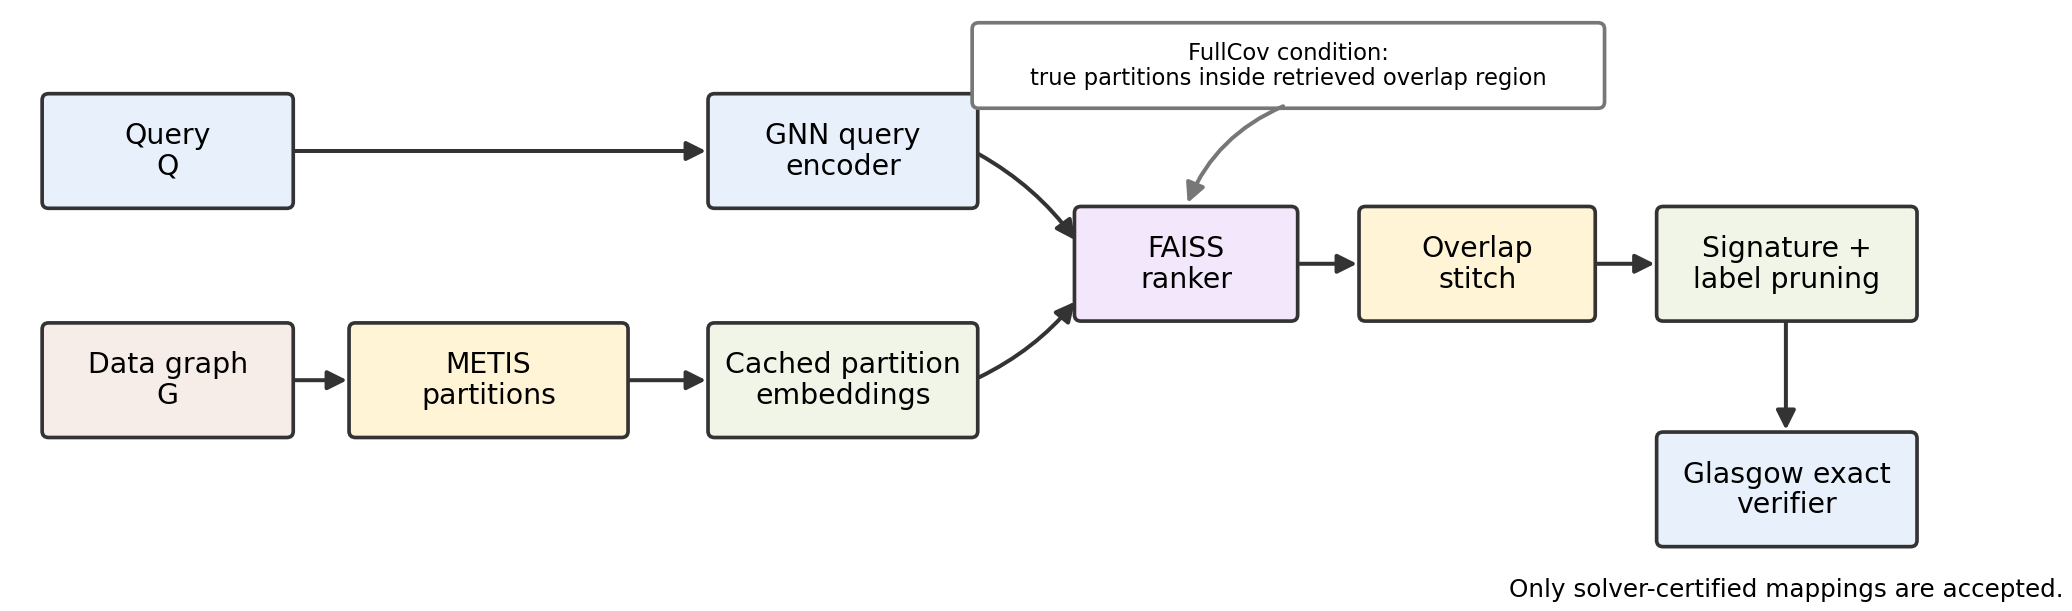
\includegraphics[width=\textwidth]{fig_jigsaw_pipeline.png}
\caption{\textbf{Jigsaw pipeline.} The learned component ranks partitions, but the only accepting step is Glasgow verification inside the stitched candidate graph. FullCov is the condition under which the candidate contains every partition needed by the planted match.}
\label{fig:pipeline}
\end{figure}

\paragraph{Hierarchical localization.}
The data graph is partitioned into fine and coarse METIS blocks. Fine blocks give local structure; coarse blocks are the retrieval units. For each query, Jigsaw computes an embedding $z_Q=f_\theta(Q)$ and ranks all coarse partitions by cosine similarity to cached partition embeddings. FAISS provides fast top-$K$ retrieval.

\paragraph{Overlap cascade.}
Hard partition boundaries are brittle: true query neighborhoods often cross coarse blocks. Jigsaw therefore stitches the retrieved partitions plus one-hop neighboring overlap. This increases recall before exact verification while still avoiding full-graph search.

\paragraph{Pruning and verification.}
The stitched region is filtered by typed structural signatures and exact labels before Glasgow verification. Signatures reduce the candidate domain by matching coarse type and feature fingerprints; exact labels are especially important for negative-label queries. The final answer is produced only by the exact verifier.

\paragraph{FullCov objective.}
Standard contrastive training rewards high average similarity to positives, which can still leave one required partition ranked too low. Jigsaw optimizes the bottleneck. For each query $Q_i$, let $\mathcal{P}_i$ be its positive partitions and let $s_{ij}$ be the query-partition score. The objective combines multi-positive contrastive learning with a weak-positive term:
\begin{equation}
\mathcal{L}_{\mathrm{weak}}(i)=-\log
\frac{\exp(\min_{p\in\mathcal{P}_i}s_{ip}/\tau)}
{\exp(\min_{p\in\mathcal{P}_i}s_{ip}/\tau)+\sum_{n\in\mathcal{N}_i}\exp(s_{in}/\tau)}.
\end{equation}
Additional CVaR and barrier terms penalize positives that fall below the chosen retrieval budget. Partition embeddings are refreshed from cache, with live re-encoding of required positives so the weakest positive receives a usable gradient. The Arxiv ablation in Table~\ref{tab:loss_ablation} isolates the value of this objective under matched training budgets.

\paragraph{Why the weakest positive.}
The choice of the $\min$ (and its CVaR relaxation) over positives follows directly from the metric. $\mathrm{FullCov@K}(Q)=\mathbf{1}[\mathcal{T}(Q)\subseteq R_K(Q)]$ is a \emph{conjunction} over the required partitions: it succeeds only if \emph{every} $p\in\mathcal{P}_i$ is ranked within $K$. Its failure is therefore governed by the single worst-ranked required partition, i.e.\ by $\min_{p\in\mathcal{P}_i} s_{ip}$, not by the average positive score that standard contrastive learning maximizes. Optimizing the average can raise mean recall while leaving one required partition below the budget, which is exactly the failure exact verification cannot tolerate. The weak-positive term targets that bottleneck directly; CVaR (the mean of the worst $\alpha$-fraction of positives) is a smooth surrogate for the non-differentiable $\min$ that spreads gradient over the few hardest required partitions rather than a single argmin. This is why, in Table~\ref{tab:loss_ablation}, the objective improves fixed-budget FullCov most at the operating points the cascade actually uses, even though average recall barely moves.

\subsection{Encoder Architecture and Training Interface}

\begin{figure}[H]
\centering
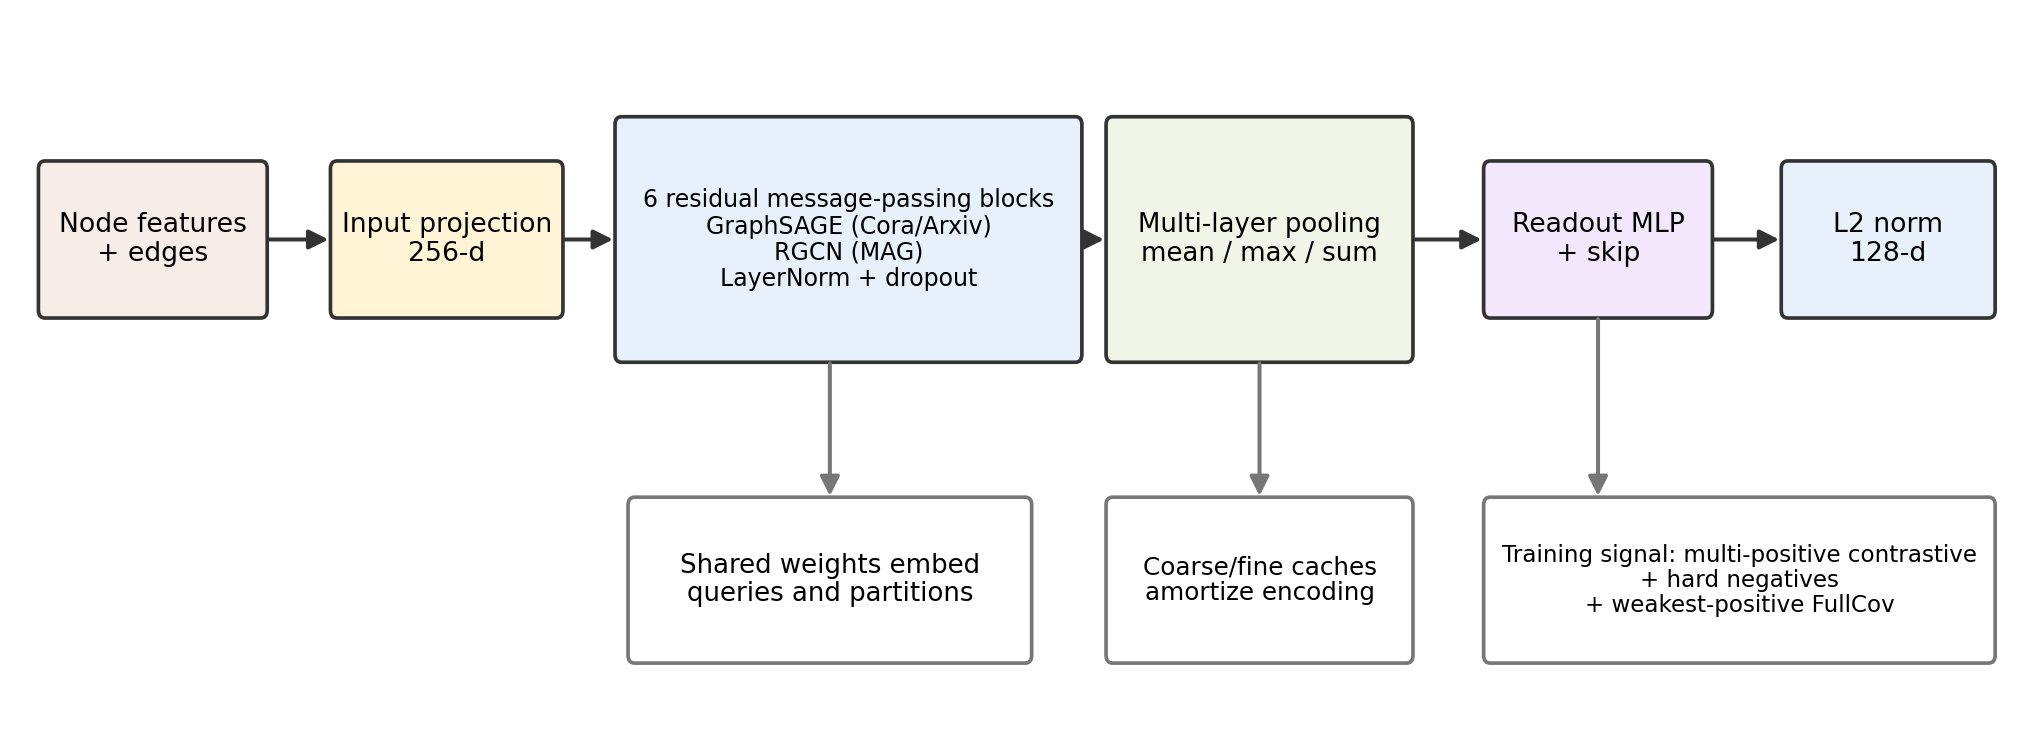
\includegraphics[width=\textwidth]{fig_encoder_architecture.png}
\caption{\textbf{Retrieval encoder.} Cora and Arxiv use a six-block residual GraphSAGE encoder; MAG uses the same six-block residual architecture with relation-aware RGCN layers. The same encoder embeds queries and cached graph partitions into a normalized 128-dimensional space.}
\label{fig:encoder}
\end{figure}

The encoder is intentionally shared between query graphs and partition graphs. Input node features are projected to a 256-dimensional hidden space, passed through six residual message-passing blocks, normalized with LayerNorm, and read out with multi-layer global mean, max, and sum pooling. The readout is an MLP plus a skip projection, followed by L2 normalization to produce a 128-dimensional retrieval vector. This matters because the retrieval problem is not node alignment; it is region localization. The model must place a query near every partition needed for exact verification, including the weakest or farthest true partition.

For Cora and Arxiv, the message-passing block is GraphSAGE ($\mathtt{SAGEConv}$); on these label-rich graphs a matched objective ablation finds GraphSAGE at least as strong as a GIN encoder at the fixed budgets the cascade uses (FullCov@20/50 in particular), so we adopt it as the homogeneous-graph encoder. OGBN-MAG is a \emph{heterogeneous} academic graph (paper, author, institution, and field-of-study nodes joined by typed relations); we flatten it to a single node/edge index for the pipeline but \emph{retain} node types and relation (edge) types and model them with a relation-aware six-layer RGCN ($\mathtt{RGCNConv}$ with per-relation bases over $2R$ relations after symmetrization). Because OGBN-MAG supplies input features only on paper nodes, non-paper nodes receive node-type one-hot and per-relation-degree features, so the retriever reasons over typed structure rather than discarding it. Both encoders use the same retrieval interface: cached fine and coarse partition embeddings are compared to query embeddings, and positive partitions can be live-reencoded during training so that coverage gradients update required positives instead of treating the entire partition bank as stale constants.

Training uses three complementary signals. First, multi-positive contrastive learning pulls a query toward all coarse partitions touched by the planted match. Second, hard negatives keep nearby but incorrect partitions separated. Third, the FullCov-oriented coverage term penalizes the weakest required positive, because downstream exact verification fails if even one necessary partition is missing. In the final MAG training run, the selected checkpoint is the validation-best FullCov model rather than merely the final epoch checkpoint; this is why the final benchmark bundle separates \texttt{mag\_rgcn\_best} production rows from \texttt{mag\_rgcn\_final} diagnostic rows.

\subsection{Why Exactness Is Conditional}

The architecture does not make the neural retriever an exact solver. It only proposes a candidate boundary. Once the candidate graph $G_C$ is constructed, Glasgow gives exact answers for $G_C$. Therefore a positive query can fail for two different reasons: either the retrieval boundary does not contain the planted solution, or the candidate becomes too large and the solver times out. The benchmark records both with candidate coverage diagnostics, timeout counts, and solved-by-budget curves. Negative queries test a different property: whether the candidate construction plus exact verifier returns no match when the generator intended the query to be impossible.

\section{Experimental Protocol}

\paragraph{Datasets.}
We evaluate Cora~\cite{ref_cora}, OGBN-Arxiv~\cite{ref_ogb}, and the full heterogeneous OGBN-MAG. Cora is small enough for exact timing sanity checks. Arxiv is the main medium-scale benchmark. OGBN-MAG is a large heterogeneous graph (1{,}939{,}743 nodes across four node types joined by typed relations) and stresses the approach with both scale and relation-aware structure; it is modeled relation-aware (RGCN over retained node/edge types), not collapsed to an attribute-only homogeneous graph.

\paragraph{Label granularity.} The exact verifier matches on discrete vertex labels obtained by hashing each node's full attribute vector ($\sigma(v)=\mathrm{md5}(x_v)\bmod 10^{6}$), which is highly---though not perfectly---discriminative: the $10^{6}$ codebook admits collisions across the ${\sim}736$K featured MAG nodes, so a returned match is exact with respect to \emph{hashed-label} semantics rather than raw attribute equality (this is the one benchmark-level false positive we report per MAG method, Section~\ref{sec:limits}). The discretized labels are nonetheless highly selective, and this is the dominant reason every retrieval policy recovers all Cora and Arxiv positives once coverage is met: we describe these as \emph{label-rich} benchmarks and treat retrieval as a candidate-cost lever rather than an accuracy lever. A coarser, more realistic labeling would weaken pruning and make retrieval correspondingly more decisive -- the planted-benchmark limitation we discuss in Section~\ref{sec:limits}.

\paragraph{Connected-positive protocol.}
All positive query families are generated as \emph{connected} subgraphs: an earlier multi-region generator could emit disconnected positives, which we corrected so that every multi-fine and multi-coarse positive is a single connected planted match. All rows in this paper use these connected reruns (the MAG connected refresh is merged into the canonical grid); we state this protocol once here rather than repeating it per result.

\paragraph{Queries and retrieval policies.}
The production matrix uses two query seeds (20260607 and 20260608), three target sizes (20, 50, 100), and 50 queries per type/size/seed. Positive query families are single-partition, multi-fine, K-hop, degree K-hop, random walk, and multi-coarse. Negative families are negative-label and negative-structure. The benchmark compares six policies because each isolates a different failure mode. \textbf{Jigsaw} ranks coarse partitions with the learned GraphSAGE/RGCN retriever (GraphSAGE on Cora/Arxiv, RGCN on MAG). \textbf{MeanFeat} ranks partitions by cosine similarity between query mean node features and cached partition mean features. \textbf{Mean-RRF} is reciprocal-rank fusion of the learned Jigsaw ranking and the MeanFeat ranking; it is therefore a second configuration of Jigsaw's own retriever, not a purely nonparametric baseline. \textbf{TopoFeat} ranks by coarse structural descriptors such as size, internal edges, average degree, density, and boundary ratio. \textbf{Random} tests whether labels and pruning alone can rescue an uninformed ranker. \textbf{FilterAll} sends all partitions into pruning and verification; it is a recall ceiling and debugging control, not a scalable retriever.

\paragraph{Partition and overlap scale.}
Tables~\ref{tab:partition_sizes} and~\ref{tab:partition_overlap} report the hierarchy used by the corrected overlap-cascade artifacts. Coarse partitions are the units ranked by retrieval, while fine partitions support local overlap and bridge construction. The partitions are deliberately balanced: MAG has 2,000 coarse partitions with median size 969 nodes and 10,000 fine partitions with median size 194 nodes. It is important to state the overlap operator precisely, because a coarse measurement can be alarming. The operator adds, for a selected partition $p$, only the \emph{boundary nodes} of other partitions that share an edge with $p$ -- not the entire bordering partitions. On MAG a median partition borders 948 of the 2{,}000 coarse partitions, but the boundary nodes it actually admits number only about 4{,}252; the expanded region for a single selected partition is therefore about 5{,}228 nodes (a $5.4\times$ expansion over the 969-node partition), not the $\approx$921K one would get by taking the union of every bordering partition in full. That 921K figure is a loose reachability bound that the operator never realizes. Candidate size grows large only when the cascade \emph{unions} the boundary overlaps of the hundreds to a thousand partitions in the retrieval budget, and because boundary nodes are shared across many partitions this union saturates between roughly 59\% (Jigsaw) and 83\% (uninformed policies) of MAG at the largest budgets. Overlap is thus a per-partition recall-expansion mechanism that is individually tight but collectively broad; the verifier only sees the much smaller pruned candidate graph reported in Table~\ref{tab:production_matrix}, and Section~\ref{sec:shrinkage} dissects exactly how much each cascade stage removes.

\begin{table}[H]
\centering
\caption{\textbf{Partition balance.} Coarse partitions are ranked by retrieval; fine partitions support local overlap and bridge construction. Node counts are per partition.}
\label{tab:partition_sizes}
\scriptsize
\resizebox{\textwidth}{!}{\begin{tabular}{llrrrrrrr}
\toprule
\textbf{Dataset} & \textbf{Level} & \textbf{Graph nodes} & \textbf{Parts} & \textbf{Min} & \textbf{Median} & \textbf{Mean} & \textbf{P90} & \textbf{Max} \\
\midrule
Cora & Coarse & 19,793 & 20 & 962 & 986 & 989.6 & 1,018 & 1,019 \\
Cora & Fine & 19,793 & 100 & 190 & 197 & 197.9 & 204 & 205 \\
Arxiv & Coarse & 169,343 & 200 & 822 & 846 & 846.7 & 872 & 872 \\
Arxiv & Fine & 169,343 & 1,000 & 153 & 169 & 169.3 & 175 & 195 \\
MAG & Coarse & 1,939,743 & 2,000 & 876 & 969 & 969.9 & 999 & 999 \\
MAG & Fine & 1,939,743 & 10,000 & 170 & 194 & 194.0 & 200 & 210 \\
\bottomrule
\end{tabular}
}
\end{table}

\begin{table}[H]
\centering
\caption{\textbf{Overlap expansion scale, stated precisely.} ``+Boundary overlap'' is the median number of boundary nodes the operator actually admits for one selected partition; ``Expanded part'' is partition plus boundary overlap (with the multiple over the bare partition). ``Neighbor parts'' counts the partitions a part borders. ``Loose union bound'' is the median size if one instead took every bordering partition in full -- a reachability bound the operator never realizes, and the source of the misleadingly large ``whole-graph'' impression. The realized per-partition overlap is small ($5.4\times$ on MAG); breadth arises only from unioning over the retrieval budget.}
\label{tab:partition_overlap}
\footnotesize
\resizebox{\textwidth}{!}{\begin{tabular}{lrrrrrr}
\toprule
\textbf{Dataset} & \textbf{Coarse parts} & \shortstack{\textbf{Partition}\\\textbf{nodes (med)}} & \shortstack{\textbf{+Boundary}\\\textbf{overlap (med)}} & \shortstack{\textbf{Expanded part}\\\textbf{(med / $\times$)}} & \shortstack{\textbf{Neighbor parts}\\\textbf{med / max}} & \shortstack{\textbf{Loose union}\\\textbf{bound (med)}} \\
\midrule
Cora  & 20    & 986 & 534   & 1,533 / 1.6$\times$ & 18 / 19    & 18,820 \\
Arxiv & 200   & 846 & 1,606 & 2,470 / 2.9$\times$ & 135 / 173  & 115,004 \\
MAG   & 2,000 & 969 & 4,252 & 5,228 / 5.4$\times$ & 948 / 1,999 & 921,494 \\
\bottomrule
\end{tabular}
}
\end{table}

\begin{figure}[H]
\centering
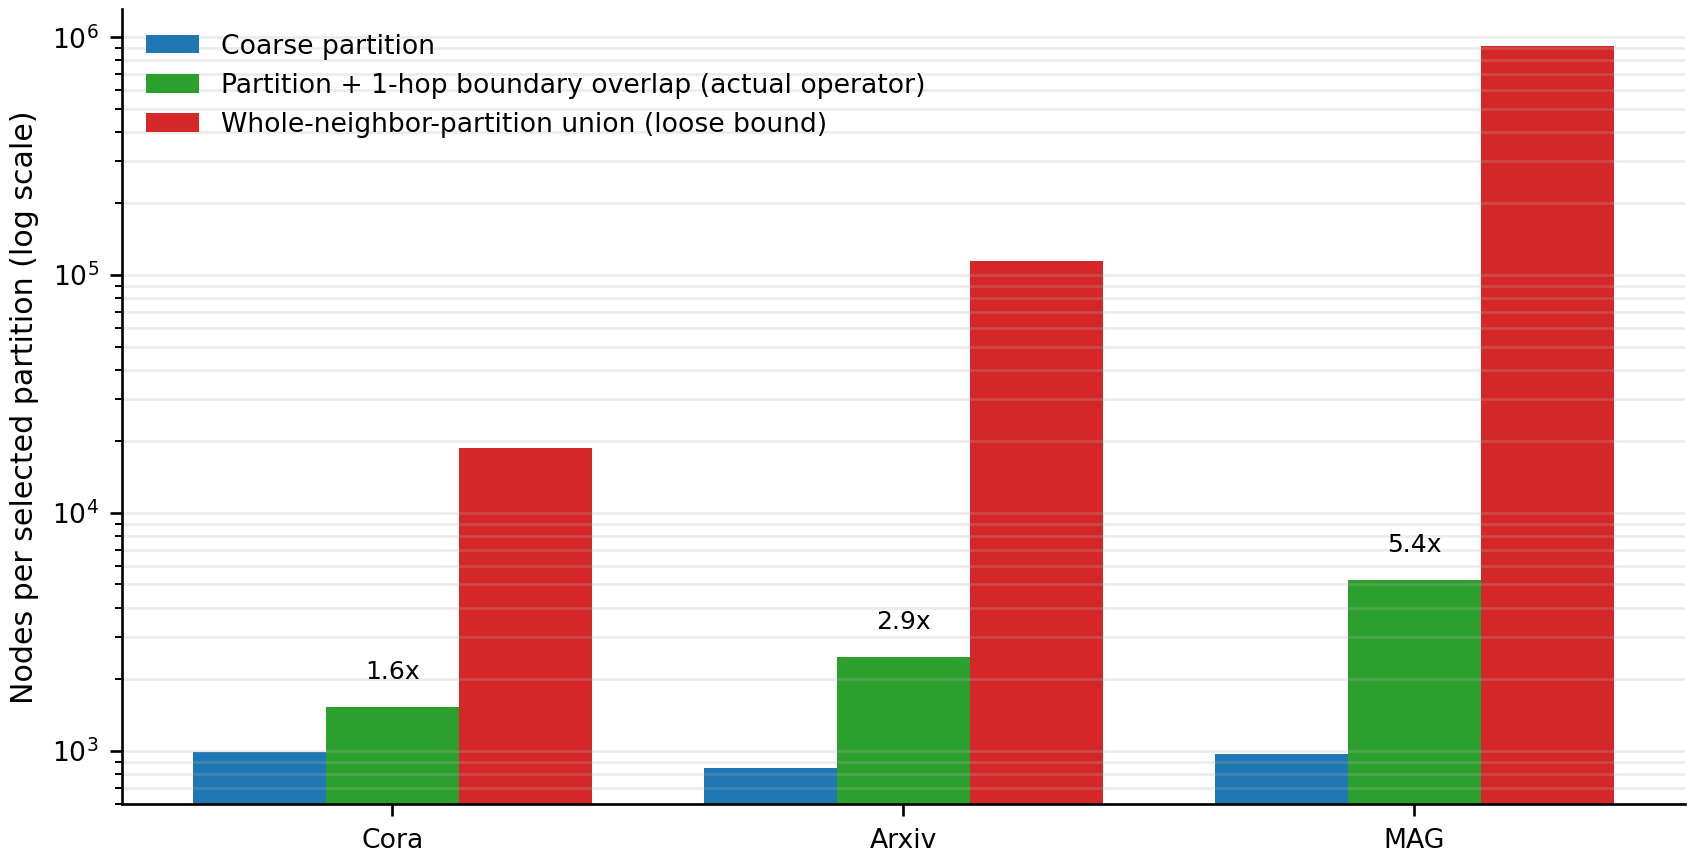
\includegraphics[width=0.82\textwidth]{fig_partition_overlap_stats.png}
\caption{\textbf{What one selected partition actually contributes (log scale).} The realized one-hop boundary overlap (green) expands a coarse partition only modestly ($1.6\times$ on Cora, $2.9\times$ on Arxiv, $5.4\times$ on MAG). The red bar is the loose union-of-whole-neighbor-partitions bound that the operator never realizes; reporting it as ``the overlap'' overstates MAG breadth by more than $170\times$. Candidate breadth instead comes from unioning these tight per-partition overlaps across the retrieval budget.}
\label{fig:partition_overlap}
\end{figure}

\paragraph{Metrics.}
For retrieval-only ablations we report FullCov@K and recall. For exact verification we report positive exact-solve rate, correct no-match rate on negatives, false positives, timeouts, candidate size, and wall-clock components. Budget columns in the released summaries are explicit: first-hit buckets are stored separately from cumulative solved-by-budget curves. The paper-facing CSV bundle is hash-manifested and separates canonical summaries from partial resume files.

\paragraph{Budget normalization.} The retrieval budget $K$ is an \emph{absolute} number of coarse partitions, but the datasets have very different partition counts (Cora 20, Arxiv 200, MAG 2{,}000). A fixed $K$ is therefore a different \emph{fraction} of each graph, so solve rates are only comparable across datasets at a matched fraction. We report two operating points: the cross-dataset-comparable \textbf{half-partition budget} ($K{=}10/100/1000$ for Cora/Arxiv/MAG) and the exhaustive \textbf{all-partition budget} ($K{=}|\mathcal{P}|$), which is the FilterAll-equivalent ceiling. MAG's headline $K{=}1000$ already \emph{is} the half-partition point; a $100\%$ rate reached only at $K{=}|\mathcal{P}|$ reflects exhaustive retrieval, not partition selection.

\paragraph{Benchmark completion and data hygiene.}
The final release bundle contains one canonical production summary per dataset and a combined all-dataset summary. Each dataset has exactly 288 production rows: 6 methods, 2 seeds, 8 query families, and 3 target sizes. Each row summarizes 50 generated logical queries, so the main production grid covers 43,200 logical method-query evaluations before budget expansion. The combined file has 864 rows and its coverage audit reports all expected cells as present. Diagnostic model variants and ablations are preserved separately so they support interpretation without inflating the main grid. Rolling Lightning resume files named \texttt{*\_partial\_per\_query.csv} are excluded from canonical summaries by default; they remain recovery artifacts, not paper evidence.

\paragraph{Implementation and reproducibility.} Partitioning uses METIS; partition and query embeddings are indexed with FAISS; exact verification uses the Glasgow Subgraph Solver, invoked on the pruned candidate graph exported in \texttt{vertexlabelledlad} format with node features discretized to integer vertex labels (Table~\ref{tab:scaling_latency} reuses the same configuration). All reported timings are per-query wall-clock on Google Cloud \texttt{CPU\_X\_8} instances (8 vCPUs), with the exact verifier run under a bounded per-query time budget (30\,s). Encoders are six residual message-passing blocks ($\mathtt{SAGEConv}$ for Cora/Arxiv, $\mathtt{RGCNConv}$ for MAG) producing $L_2$-normalized 128-dimensional embeddings. Trained encoders, query seeds, partition hierarchies, and the hash-manifested benchmark bundle will be released to support full reproduction.

\section{Results}

\subsection{FullCov Training Improves Retrieval}

Table~\ref{tab:loss_ablation} and Figure~\ref{fig:fullcov_ablation} give the matched-budget Arxiv retrieval result. All rows use the same locked K-hop query seeds and 9,000 optimizer steps. The FullCov objective improves the fixed-budget operating points most relevant to bounded exact verification.

\begin{figure}[H]
\centering
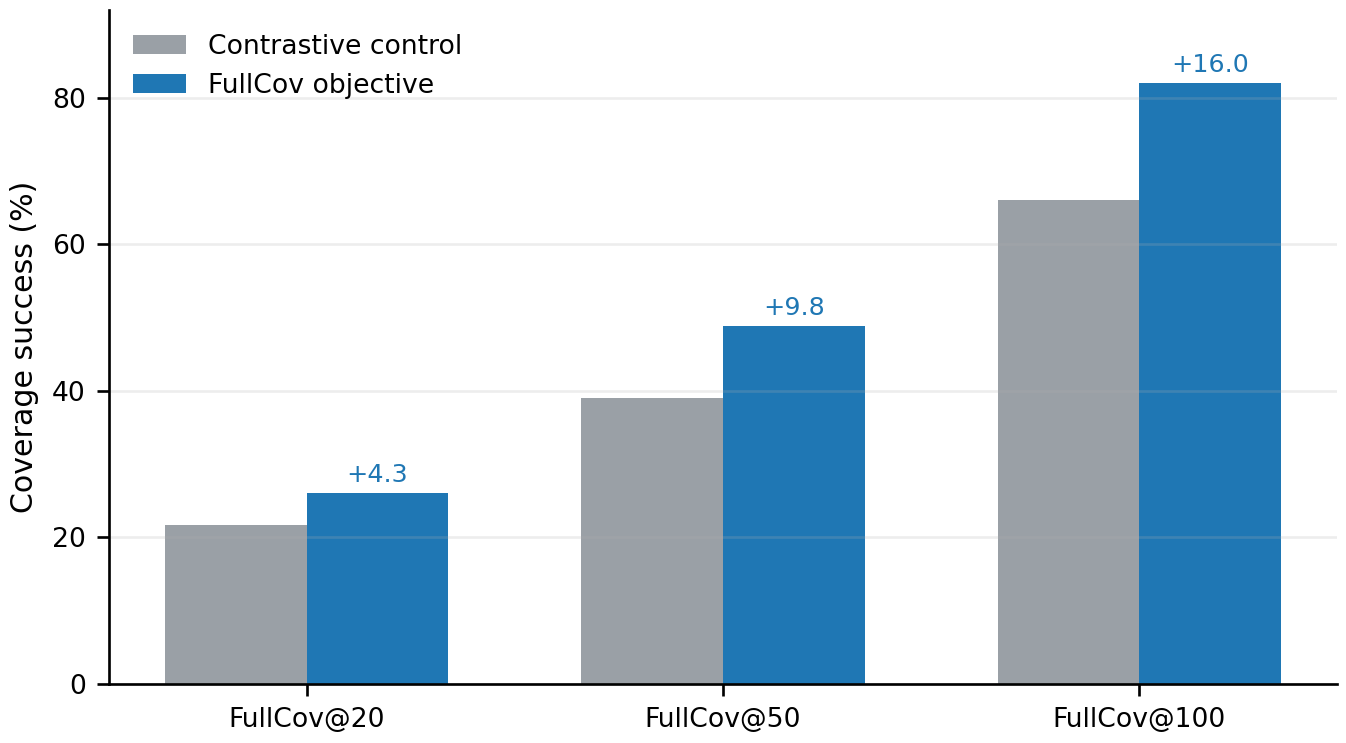
\includegraphics[width=0.72\textwidth]{fig_fullcov_ablation.png}
\caption{\textbf{FullCov objective gain.} Under matched Arxiv K-hop training conditions, directly optimizing weakest-positive coverage improves every fixed retrieval budget used by the downstream cascade.}
\label{fig:fullcov_ablation}
\end{figure}

\begin{table}[H]
\centering
\caption{\textbf{Matched Arxiv retrieval objective ablation.} Fixed retrieval budgets, two locked query seeds, two training replicates for control/final.}
\label{tab:loss_ablation}
\small
\setlength{\tabcolsep}{5pt}
\resizebox{\textwidth}{!}{%
\begin{tabular}{lcccc}
\toprule
\textbf{Objective} & \textbf{FullCov@20} & \textbf{FullCov@50} & \textbf{FullCov@100} & \textbf{Mean worst rank} \\
\midrule
Contrastive control & 21.7\% & 39.0\% & 66.0\% & 74.02 \\
FullCov objective & \textbf{26.0\%} & \textbf{48.8\%} & \textbf{82.0\%} & \textbf{58.97} \\
\midrule
McNemar $p$ & $4.6{\times}10^{-3}$ & $9.8{\times}10^{-6}$ & $4.0{\times}10^{-10}$ & -- \\
\bottomrule
\end{tabular}}
\end{table}

The effect is not a change in feasibility: the locked K-hop suite has zero queries impossible at $K=20,50,100$; average true coarse footprint is 6.37 and maximum footprint is 17. Misses are ranking errors. The objective reduces those ranking errors by explicitly optimizing the weakest required partition.

This result is the cleanest evidence for the training objective. It uses the same query seeds and training budget for the control and FullCov-aligned models, so the improvement is not explained by easier queries or longer optimization. The largest gain appears at FullCov@100, where the downstream exact verifier has enough room to benefit from better ordering but still cannot simply search the whole graph. In other words, the objective improves the operating point that the cascade actually uses.

\subsection{Three-Dataset Production Matrix}

\begin{figure}[H]
\centering
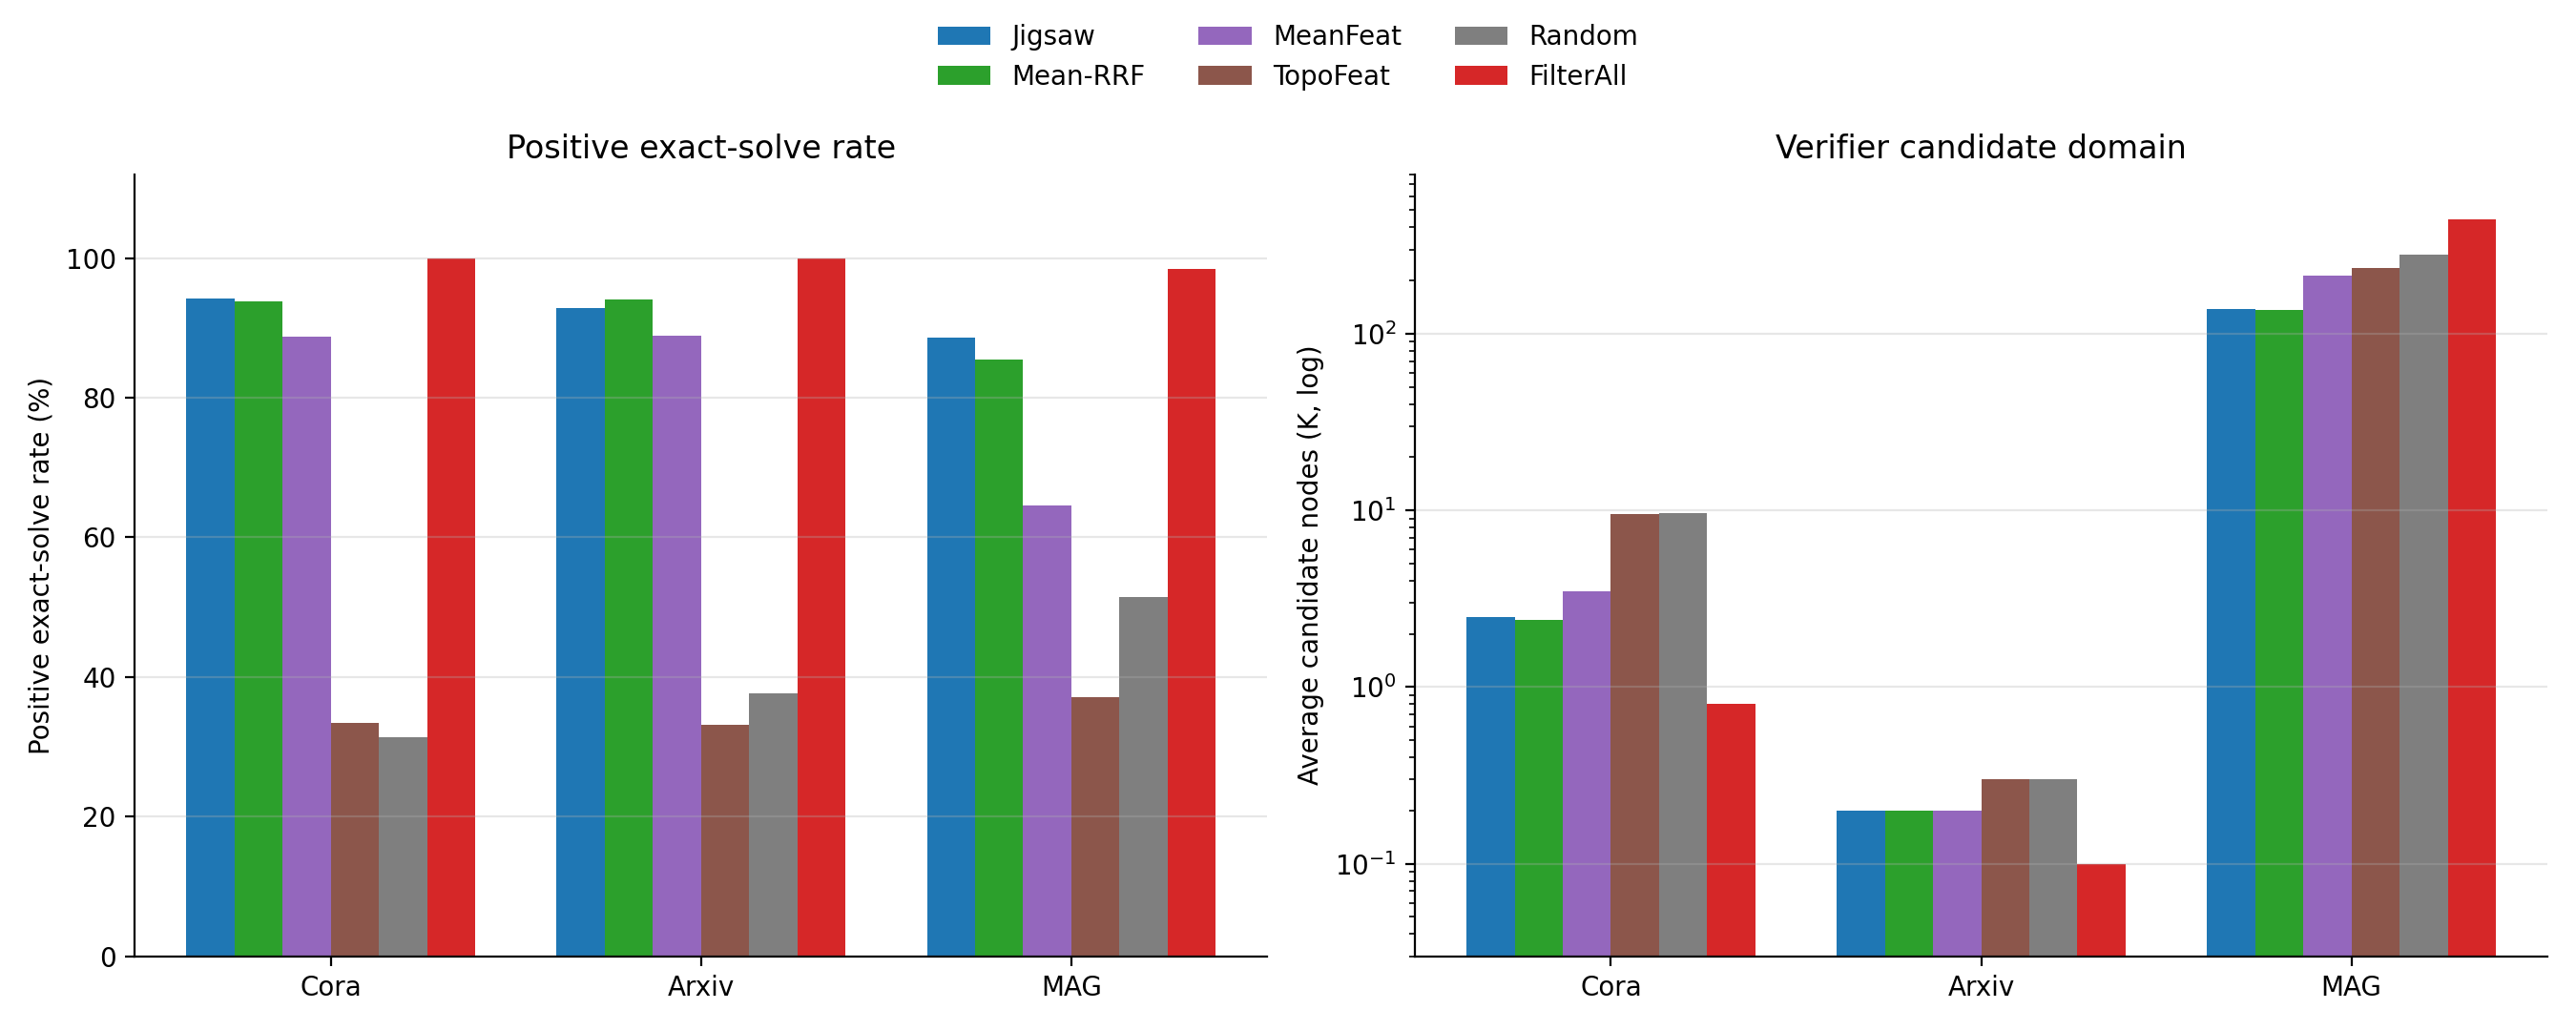
\includegraphics[width=\textwidth]{fig_production_positive_rates.png}
\caption{\textbf{Production positive exact-solve rates and candidate cost.} Production positive exact-solve rates at the matched half-partition budget ($K{=}10/100/1000$) and candidate cost. At this budget the policies separate on \emph{all three} datasets (random/topology fall to $31$--$51\%$: $31$--$38\%$ on Cora/Arxiv, $37$--$51\%$ on MAG); FilterAll (exhaustive, all partitions) is the ceiling that reaches $100\%$ on Cora/Arxiv. Right panel: verifier candidate domain (per-query average nodes).}
\label{fig:production_rates}
\end{figure}

Table~\ref{tab:production_matrix} reports the cleaned production metrics used by the manuscript. Positive queries measure exact planted-match recovery; negative queries measure correct no-match behavior. The table also includes false positives, solver timeouts, average candidate nodes, end-to-end runtime, and verifier time. Headline table values are traced in \texttt{HEADLINE\_NUMBERS.csv} and \texttt{CANONICAL\_SOURCES.md}; legacy normalized summaries are retained only for provenance and encoder-independent rows.

\begin{table}[H]
\centering
\caption{\textbf{Final production metrics across Cora, OGBN-Arxiv, and OGBN-MAG.} Pos. is planted positive exact-solve rate. Neg. is correct no-match rate. FP is false positives on negatives; TO is solver timeouts. \textbf{Pos.\ is reported at the cross-dataset-comparable half-partition retrieval budget} $K{=}10/100/1000$ for Cora/Arxiv/MAG. We use a matched \emph{fraction} because $K$ is an absolute partition count and the datasets have very different partition totals (Cora 20, Arxiv 200, MAG 2{,}000); a fixed $K$ is a different fraction of each graph, so only a matched fraction (here $50\%$) is comparable across scales. At this budget the policies separate: random/topology collapse to $31$--$51\%$ (Cora/Arxiv $31$--$38\%$, MAG $37$--$51\%$), mean-feature holds ($88.8/88.9\%$ on Cora/Arxiv), learned/fusion retrievers are strong learned configurations ($94.2/93.8$ Cora, $92.8/94.0$ Arxiv, $88.6/85.4$ MAG), and FeatureIndex is strongest on MAG under near-unique labels. $^\ddagger$\,FilterAll is budget-independent (it always sends \emph{all} partitions), i.e.\ the exhaustive ceiling; Cora/Arxiv reach $100\%$ only at that exhaustive $K{=}|\mathcal{P}|$ budget, which is \emph{not} a retrieval result. Full solved-by-$K$ curves for every budget are in Fig.~\ref{fig:budget_curves} / Section~\ref{sec:family}. Neg.\ is correct no-match rate; FP false positives on negatives; TO solver timeouts. Candidate nodes and runtimes are per-query averages over the stop-on-found cascade (verifier input medians $51/50$ nodes on Cora/Arxiv). MAG's $K{=}1000$ already \emph{is} its half-partition budget; its $88.6\%$ is distinct from the exhaustive FilterAll ceiling of $98.4\%$. The MAG Jigsaw and Mean-RRF rows use the deployed walk-aware-trained encoder (Section~\ref{sec:family}); the feature, random, topology, and FilterAll policies are encoder-independent. $^\S$\,FeatureIndex is the classical GraphGrep/gIndex-style label-coverage index (Section~\ref{sec:selectivity}); at these near-unique labels it is the strongest bounded retriever, exceeding the learned model, and was run on positives only (no-match/FP columns omitted). For the two MAG walk-aware rows the Neg.\,/\,FP\,/\,TO columns are carried from the generic-encoder benchmark (no walk-aware negative rerun exists); for the Cora/Arxiv learned rows the candidate-size and runtime columns are from the earlier full-budget run, while the overlap-retrained half-budget serve keeps the verifier input to a median $51/50$ nodes (mean $0.9$K$/88$, total $0.05/0.22$\,s).}
\label{tab:production_matrix}
\scriptsize
\setlength{\tabcolsep}{2.5pt}
\resizebox{\textwidth}{!}{%
\begin{tabular}{llrrrrrrr}
\toprule
\textbf{Dataset} & \textbf{Method} & \textbf{Pos. \%} & \textbf{Neg. \%} & \textbf{FP} & \textbf{TO} & \textbf{Cand. nodes} & \textbf{Total s} & \textbf{Solver ms} \\
\midrule
Cora & Jigsaw & 94.2 & 100.0 & 0 & 0 & 2.5K & 0.09 & 7.9 \\
Cora & Mean-RRF & 93.8 & 100.0 & 0 & 0 & 2.4K & 0.09 & 8.3 \\
Cora & MeanFeat & 88.8 & 100.0 & 0 & 0 & 3.5K & 0.11 & 7.4 \\
Cora & TopoFeat & 33.4 & 100.0 & 0 & 0 & 9.5K & 0.22 & 3.2 \\
Cora & Random & 31.3 & 100.0 & 0 & 0 & 9.6K & 0.21 & 3.2 \\
Cora & FilterAll$^\ddagger$ & 100.0 & 100.0 & 0 & 0 & 0.8K & 0.07 & 11.3 \\
\midrule
Arxiv & Jigsaw & 92.8 & 100.0 & 0 & 0 & 0.2K & 0.59 & 12.9 \\
Arxiv & Mean-RRF & 94.0 & 100.0 & 0 & 0 & 0.2K & 0.41 & 16.0 \\
Arxiv & MeanFeat & 88.9 & 100.0 & 0 & 0 & 0.2K & 0.39 & 16.5 \\
Arxiv & TopoFeat & 33.2 & 100.0 & 0 & 0 & 0.3K & 0.75 & 5.1 \\
Arxiv & Random & 37.7 & 100.0 & 0 & 0 & 0.3K & 0.77 & 5.4 \\
Arxiv & FilterAll$^\ddagger$ & 100.0 & 100.0 & 0 & 0 & 0.1K & 0.35 & 16.9 \\
\midrule
MAG & Jigsaw & \textbf{88.6} & 99.8 & 1 & 23 & 138.1K & 6.97 & 81.9 \\
MAG & Mean-RRF & 85.4 & 99.7 & 1 & 16 & 137.1K & 5.38 & 67.9 \\
MAG & FeatureIndex$^\S$ & \textbf{96.7} & -- & -- & 24 & 59.4K & 2.39 & 118.8 \\
MAG & MeanFeat & 64.6 & 99.8 & 1 & 10 & 212.1K & 8.02 & 27.5 \\
MAG & TopoFeat & 37.1 & 99.8 & 1 & 1 & 235.6K & 8.07 & 5.2 \\
MAG & Random & 51.4 & 99.8 & 1 & 8 & 282.1K & 9.54 & 19.9 \\
MAG & FilterAll$^\ddagger$ & 98.4 & 99.8 & 1 & 30 & 443.8K & 5.85 & 288.6 \\
\bottomrule
\end{tabular}}
\end{table}

Solve rate must be read against the retrieval budget. Because $K$ is an absolute partition count and Cora/Arxiv have only 20/200 coarse partitions, the headline $100\%$ on these graphs is reached \emph{only} at $K$ equal to the entire partition set -- the exhaustive, FilterAll-equivalent setting -- and is not a retrieval result. At the cross-dataset-comparable half-partition budget ($K{=}10/100/1000$), the overlap-aware GraphSAGE retriever solves $94.2\%$ (Cora) and $92.8\%$ (Arxiv); the policies separate clearly there (random and topology-only collapse to $31$--$38\%$ on these two graphs, $37$--$51\%$ on MAG), so these graphs are \emph{not} saturated once the budget is held to a sensible fraction. Crucially, the overlap-aware retraining is what closes the Arxiv gap: a retriever trained without overlap-hierarchy supervision solved only $74.1\%$ at this budget, whereas the overlap-aware model reaches $92.8\%$, nearly matching the exhaustive ceiling while seeing a median of $50$ candidate nodes; Cora was already near-saturated ($95.4\%\!\to\!94.2\%$, within noise). On these label-rich small graphs the learned retriever is competitive but not uniquely best -- Mean-RRF fusion is comparable ($93.8\%$ Cora, $94.0\%$ Arxiv) -- consistent with our framing of the retriever as a replaceable component. On candidate cost, the overlap-aware models keep the verifier input small: a median of $51$ pruned nodes on Cora and $50$ on Arxiv (mean $0.9$K and $88$).

MAG is the genuine stress case, and its $K{=}1000$ budget already \emph{is} half its 2{,}000 partitions. Random and topology-only retrieval degrade sharply, mean features help, and Jigsaw's deployed walk-aware model reaches \textbf{88.6\%} positive solves, ahead of Mean-RRF ($85.4\%$) and mean features ($64.6\%$). The learned retriever is \emph{not}, however, the strongest memory-bounded policy on this benchmark: a classical label-coverage index (\textbf{FeatureIndex}, GraphGrep/gIndex-style) reaches \textbf{96.7\%} with a \emph{smaller} candidate ($59.4$K vs $138.1$K nodes) and lower latency ($2.39$ vs $6.97$\,s), because these near-unique md5 labels make exact-label coverage a near-oracle localizer. We do not paper over this---it is the central lesson of Section~\ref{sec:selectivity}, where the index's advantage is shown to be an artifact of near-unique labels that \emph{inverts} once labels are coarse. This is not a recall win over exact matchers: once the whole graph is resident, CFL/DP-iso/GQL solve Cora/Arxiv at $100\%$ and MAG at $27/27$ under high selectivity (Table~\ref{tab:external}) -- more than Jigsaw's $88.6\%$. Jigsaw's contribution is achieving exact matching \emph{without} that residence (2.4 vs 10.2\,GB), not out-recalling a resident solver. Indeed the load-split timings show the barrier at scale is \emph{residence, not matching}: at high label selectivity CFL/DP-iso/GQL enumerate a MAG query in ${\sim}1$\,ms, and their ${\approx}8.4$\,s wall-clock is almost entirely the one-time full-graph load. We therefore make no speed claim over resident matchers -- for a resident, repeated-query workload their match is far faster; Jigsaw targets the regime where the graph cannot or should not be held resident, and where the CP verifier does not finish at all. Exhaustive FilterAll reaches $98.4\%$ but hands the verifier all partitions, so it is the recall ceiling rather than a scalable policy. Crucially, Jigsaw admits only about $138.1$K of the $1{,}939{,}743$ MAG nodes into its pruned candidate ($\sim$7\%, a $14.0\times$ reduction over the full graph and $3.2\times$ fewer than FilterAll's $443.8$K), which component decomposition then reduces to solver inputs of median ${\sim}100$ nodes, at far lower verifier time ($82$ vs $289$\,ms); this candidate reduction is what converts the direct solver's $0/15$ into a tractable $88.6\%$, though candidate construction remains the dominant cost. \textbf{Moreover, the cascade never holds the whole graph resident.} It admits partitions one at a time and prunes on node-ID and label sets before ever materializing edges, so peak memory tracks the pruned candidate frontier, not the target. A conservative streaming serve that caps the resident partition cache (eight partitions) and fetches survivor edges in a second pass makes this concrete: across a 54-query MAG grid (all six families, three sizes) it peaks at \textbf{2.4\,GB}, against \textbf{10.2\,GB} to hold MAG resident for a direct solve -- a $4.2\times$ reduction -- while recovering $46/54$ planted matches (all 36 easy-family queries; the 8 misses are all random-walk or multi-coarse, retrieval misses matching the production bottleneck) and handing the solver components of median $110$ nodes (max $9{,}497$) that solve in $5$\,ms--$8.4$\,s.

\begin{figure}[H]
\centering
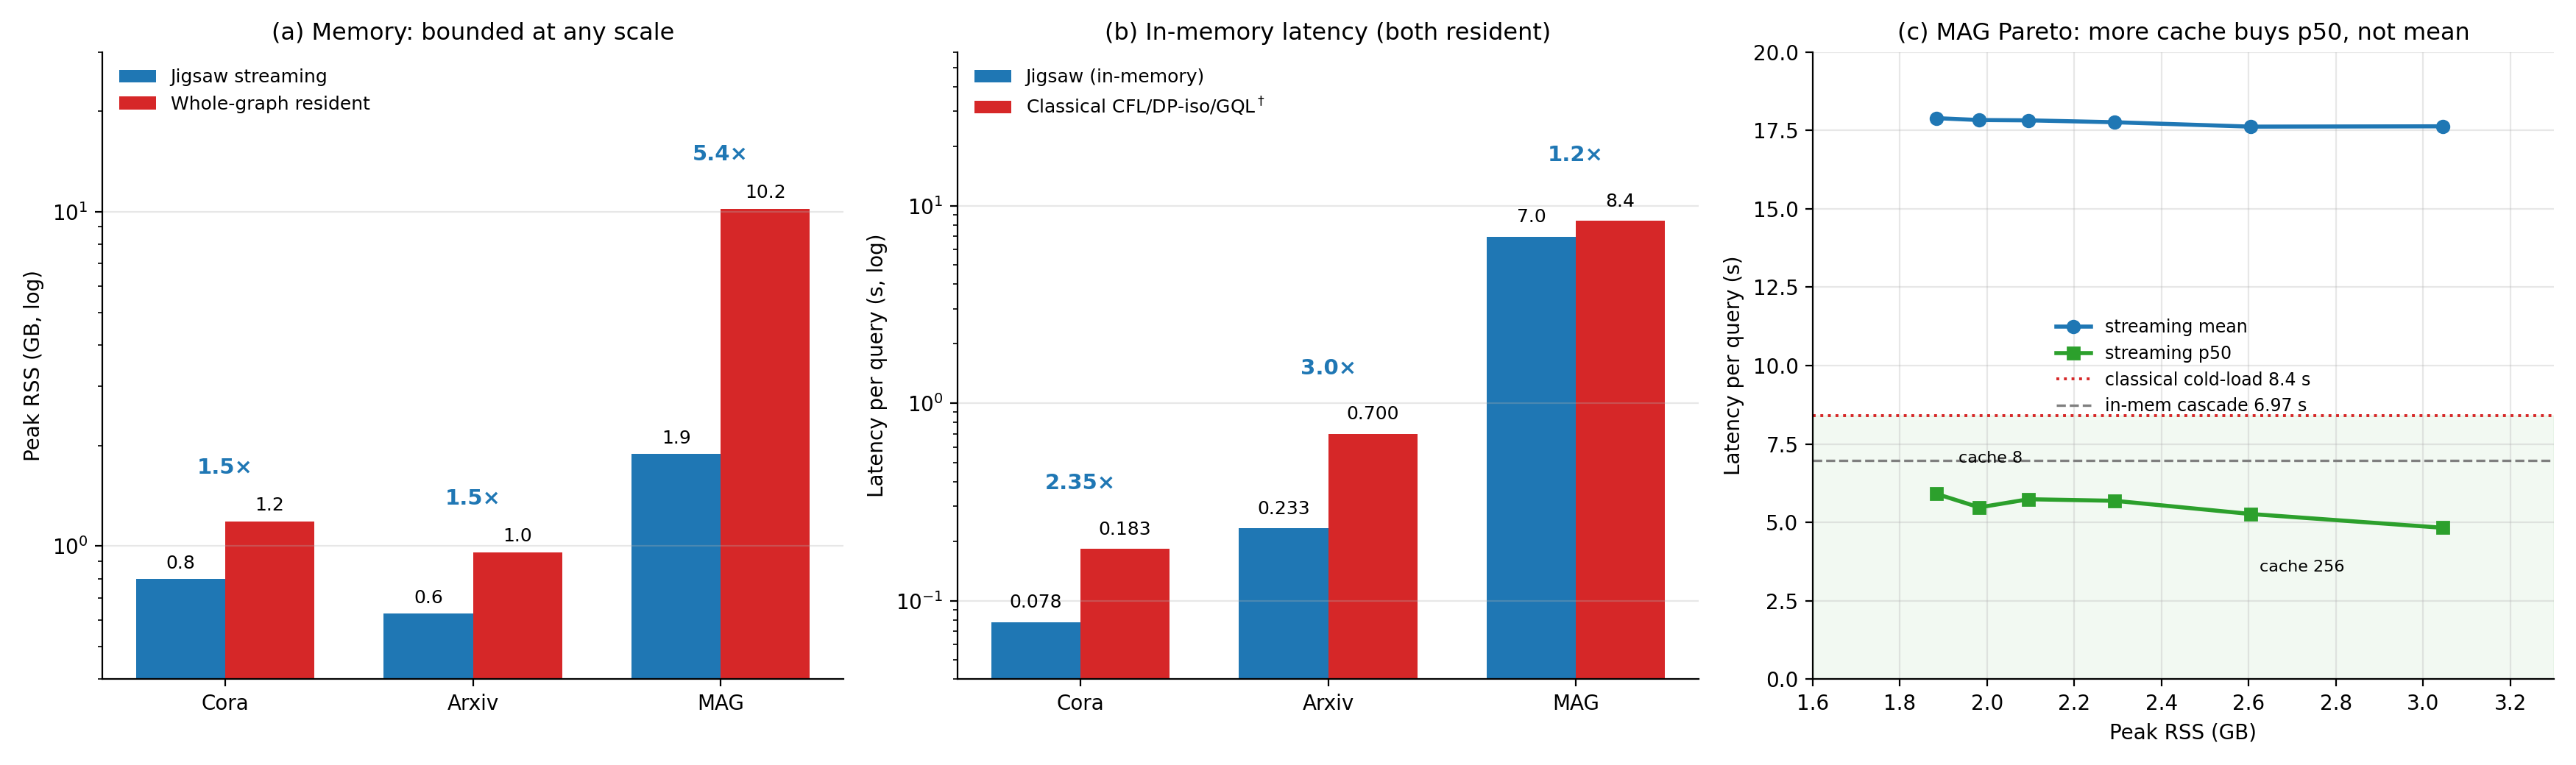
\includegraphics[width=\textwidth]{fig_memory_latency.png}
\caption{\textbf{Memory is the clean win; cold-load latency is competitive but load-dominated; the tradeoff is tunable.} \textbf{(a)} Peak RSS, streaming serve vs.\ whole-graph residence -- bounded on every dataset, $5.4\times$ smaller on MAG ($1.9$ vs $10.2$\,GB). \textbf{(b)} Cold-load end-to-end latency, Jigsaw cascade vs.\ classical CFL/DP-iso/GQL: $2.35$/$3.0$/$1.2\times$ faster on Cora/Arxiv/MAG. This edge is \emph{load avoidance}, not faster resident matching -- the classical wall-clock is dominated by per-query full-graph load ($^\dagger$MAG's ${\approx}8.4$\,s is almost all load, ${\sim}1$\,ms if kept resident), so we make no raw-speed claim. \textbf{(c)} The MAG memory$\leftrightarrow$latency frontier as the streaming cache grows ($8{\to}256$ partitions): more memory buys down the median (p50 $5.9{\to}4.8$\,s, below the $8.4$\,s cold-load) but the mean stays flat ($17.9{\to}17.6$\,s), dominated by a hard-query I/O tail rather than cache re-reads. Jigsaw lets the operator pick a point on this frontier that all-or-nothing resident matchers cannot offer.}
\label{fig:memory_latency}
\end{figure}

\textbf{The memory saving is tunable, and it -- not latency -- is the contribution.} Sweeping the streaming serve's resident-partition cache traces a memory$\leftrightarrow$latency frontier (Fig.~\ref{fig:memory_latency}) that an all-or-nothing classical matcher cannot offer: it is either whole-graph-resident and fast, or reloads the full graph per query. On MAG the optimized serve operates from $1.9$\,GB (cache 8) to $3.0$\,GB (cache 256) -- always $3$--$5\times$ under the $10.2$\,GB resident footprint -- at a median per-query latency of $4.8$--$5.9$\,s, below the ${\approx}8.4$\,s a cold classical solver pays to load MAG once. (The $2.4$\,GB headline quoted earlier is this same serve before the fetch/prune vectorizations; those optimizations lower the $8$-partition point to $1.9$\,GB.) We deliberately do \emph{not} read this as a speed win: the mean latency ($17.6$\,s) is dominated by a hard-query tail and does \emph{not} fall with more cache, and a resident classical solver amortizes its one-time load to ${\sim}1$\,ms and is far faster on a repeated-query workload. The defensible claim is narrower: Jigsaw performs exact matching under a \emph{chosen} memory budget that resident solvers cannot meet, and lets the operator pick a point on the frontier rather than pay full residence. On the small graphs the frontier is flat -- Cora and Arxiv stream at $0.8$ and $0.6$\,GB (vs.\ $1.2$ and $1.0$\,GB resident) at ${\approx}56$--$67$ and ${\approx}250$--$370$\,ms across the cache sweep -- because they fit in memory anyway; the tradeoff only becomes meaningful at MAG scale.

\begin{figure}[H]
\centering
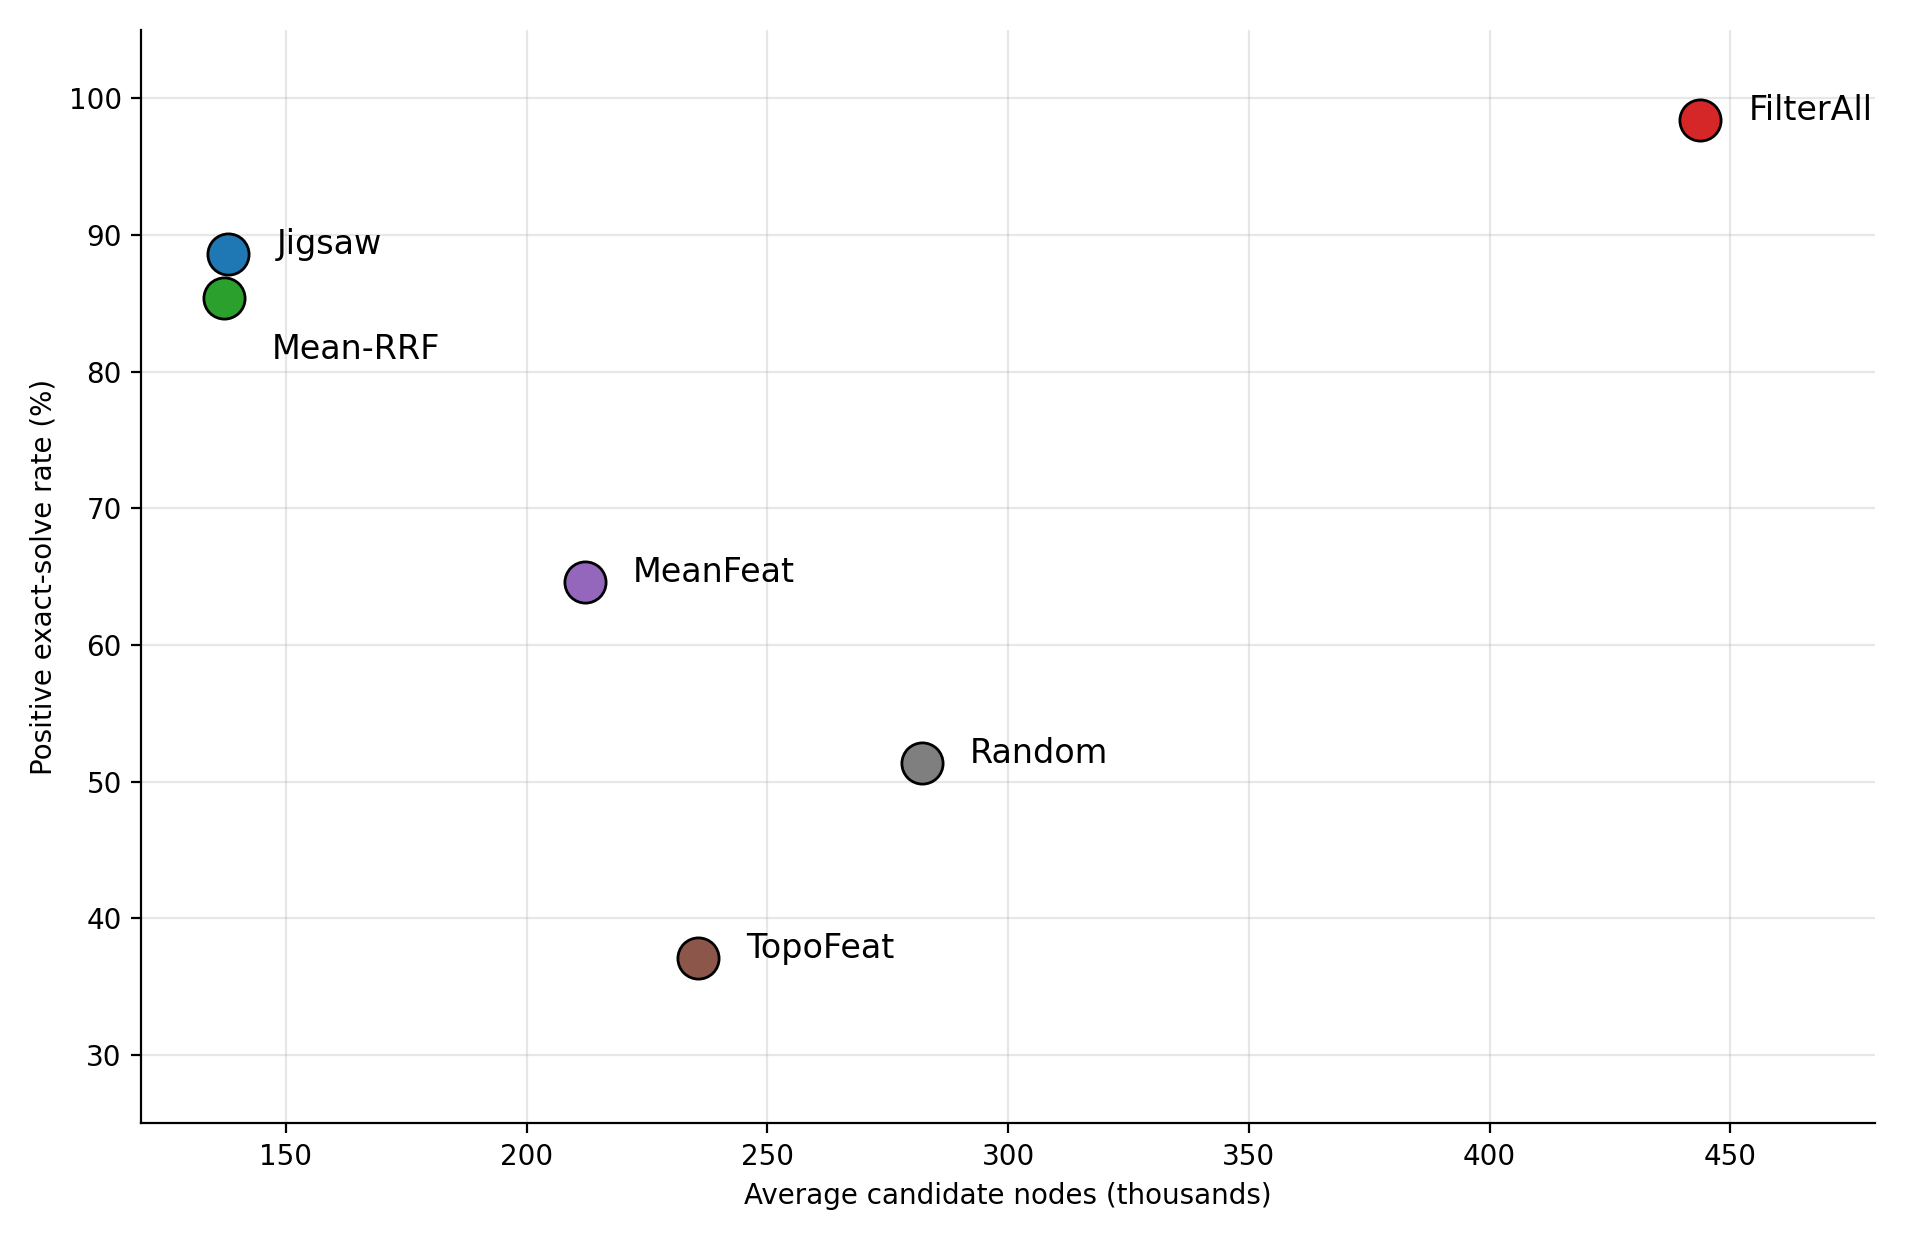
\includegraphics[width=0.86\textwidth]{fig_mag_tradeoff.png}
\caption{\textbf{MAG tradeoff.} MAG is the production dataset where retrieval policies separate sharply. FeatureIndex is strongest under near-unique labels; FilterAll is the exhaustive ceiling; learned Jigsaw is a memory-bounded operating point that uses less than half the candidate nodes of FilterAll.}
\label{fig:mag_tradeoff}
\end{figure}

The MAG result is the most important systems result in the paper. It has a clear lower bound: \emph{direct exact matching on the full graph with no retrieval} (the query handed to Glasgow against the entire 1.9M-node MAG target) solves \textbf{0 of 15} sampled K-hop queries, every one exhausting the time budget (median ${\approx}25$\,s per query including target loading). The direct Glasgow solve is therefore infeasible at this scale -- retrieval is a prerequisite for the CP solver, not an optimization (scalable filter-and-verify matchers solve MAG once the whole graph is loaded at high selectivity, Table~\ref{tab:external}, but require full residence and degrade at low selectivity) -- which is the gap every policy in Table~\ref{tab:production_matrix} is measured against. This crossover is not unique to MAG: the identical direct solver solves all 15 Cora queries but collapses to \textbf{0 of 15} on OGBN-Arxiv, while the Jigsaw cascade stays feasible by handing the verifier a pruned candidate of $\sim\!50$ nodes instead of the full $169$K. The retriever is therefore a component on a recall-vs-cost frontier. FeatureIndex is the strongest bounded policy under near-unique MAG labels; FilterAll is the recall ceiling at the highest verifier cost; the learned retriever is a useful memory-bounded operating point, especially once labels coarsen, and sends the verifier $3.2\times$ fewer candidate nodes than FilterAll.

\begin{figure}[H]
\centering
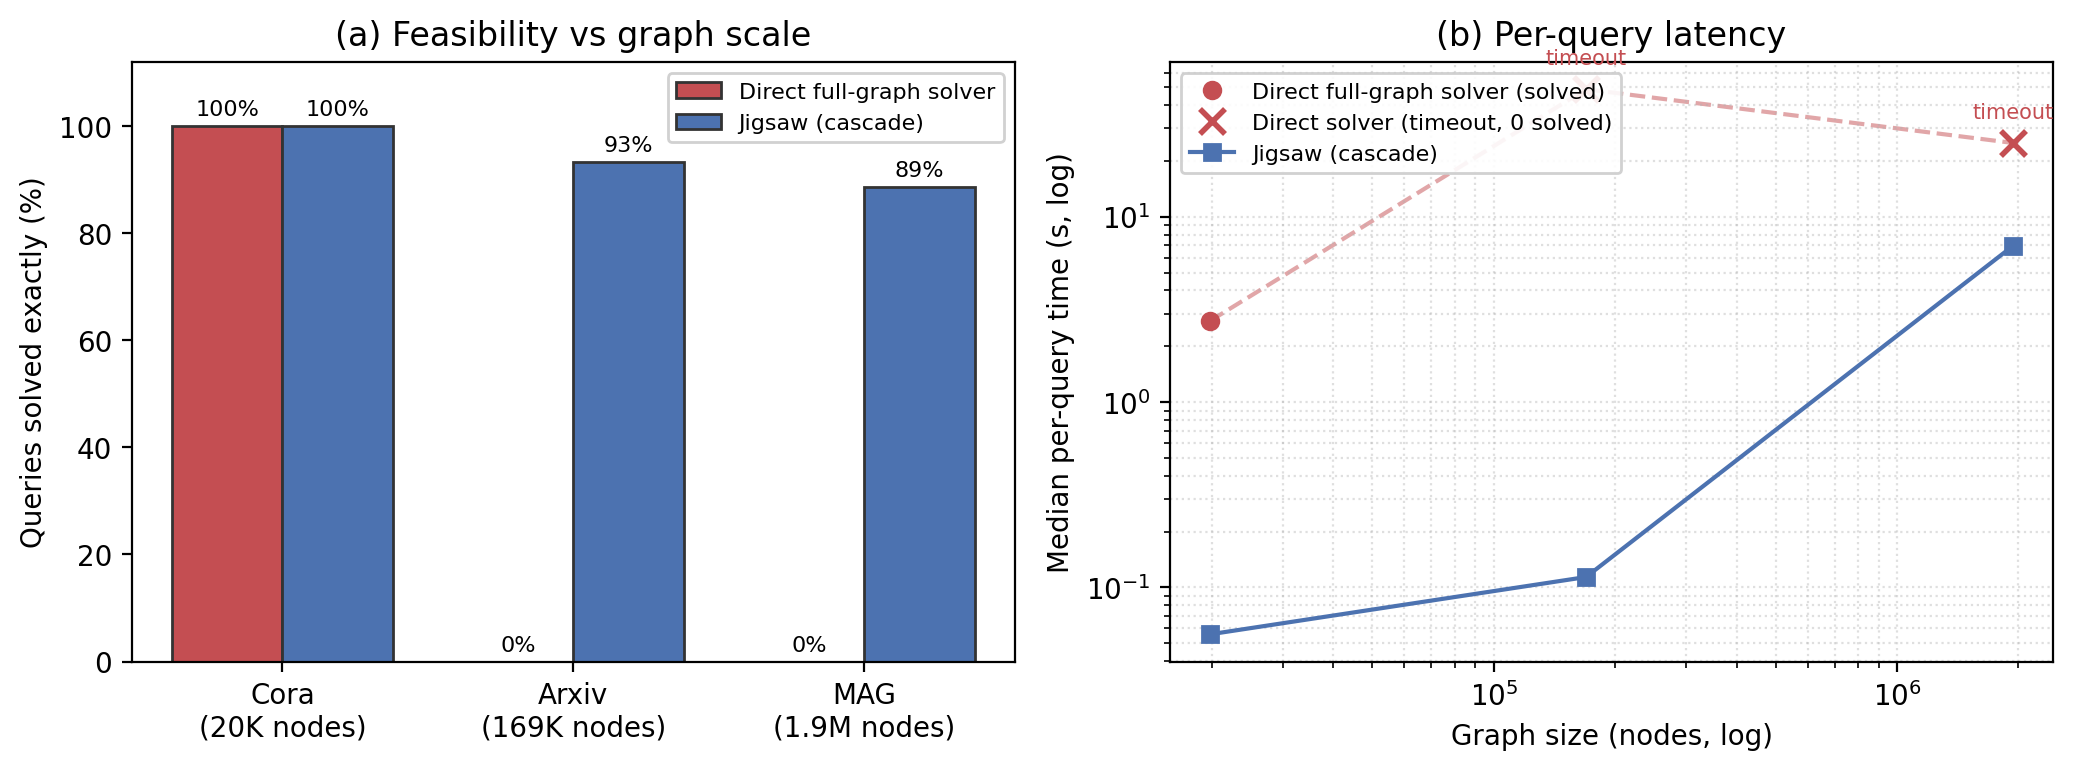
\includegraphics[width=0.82\textwidth]{fig_scaling_feasibility.png}
\caption{\textbf{Jigsaw makes the exact solver's domain tractable.} (a) Feasibility vs.\ graph scale: the direct full-graph solver clears all Cora queries but solves \emph{none} at Arxiv (169K) or MAG (1.9M) scale, while the Jigsaw cascade stays feasible throughout (100/93/89\%). (b) Per-query latency (log--log): the direct solver is censored at its time budget (X = timeout, 0 solved) for Arxiv and MAG; Jigsaw runs one-to-three orders of magnitude faster because the verifier sees only the retrieved-and-pruned candidate. Matched K-hop queries; numbers in Table~\ref{tab:scaling_latency}.}
\label{fig:scaling}
\end{figure}

\begin{table}[t]
\centering
\caption{\textbf{Scaling and latency: direct full-graph solver vs.\ Jigsaw cascade}, on matched K-hop queries (seed 20260607, target sizes 20/50/100, 5 each = 15 queries per dataset; MAG cascade is the production-matrix neural retriever over its eight query families). The direct solver hands Glasgow the entire graph; Jigsaw hands it the retrieved, overlapped, and pruned candidate. ``Median time'' is wall-clock per query (retrieval${+}$candidate${+}$solve for Jigsaw; solve for the direct baseline). $^\dagger$ The direct solver is given the same 30\,s solve budget as the verifier; reported times are wall-clock to abort, which exceeds the request because Glasgow does not preempt cleanly (${\approx}49$\,s on Arxiv; the MAG ${\approx}25$\,s is dominated by loading the 1.9M-node target before abort). The run is aborted with no match returned. $^\ast$ The MAG cascade cell is the per-query \emph{mean} total from the production matrix (Table~\ref{tab:production_matrix}); the Cora/Arxiv cascade cells are true medians.}
\label{tab:scaling_latency}
\small
\begin{tabular}{l r c r c r r}
\toprule
 & & \multicolumn{2}{c}{Direct full-graph solver} & \multicolumn{2}{c}{Jigsaw cascade} & Cand.\ \\
\cmidrule(lr){3-4}\cmidrule(lr){5-6}
Dataset & Nodes & Solved & Med.\ time & Solved & Med.\ time & nodes \\
\midrule
Cora  & 19.8K & 15/15 & $2.74$\,s & 15/15 & $\mathbf{0.06}$\,s & 51 \\
Arxiv & 169K  & \textbf{0/15}$^\dagger$ & ${\approx}49$\,s & 14/15 & $\mathbf{0.11}$\,s & 50 \\
MAG   & 1.9M  & \textbf{0/15}$^\dagger$ & ${\approx}25$\,s & 88.6\% & $6.97$\,s$^\ast$ & -- \\
\bottomrule
\end{tabular}
\end{table}

\paragraph{Statistical significance.}
Table~\ref{tab:significance} reports bootstrap 95\% confidence intervals on the MAG positive solve rate (n${=}1800$ queries per method) and paired exact-McNemar tests, pairing per query so that wins/losses count only the queries two policies decide differently. Among the retrieval \emph{components} we evaluate, the FullCov-trained retriever significantly outperforms the other learned and feature retrievers (Mean-RRF, re-evaluated under the same walk-aware encoder, $92$ vs $35$, $p{=}4.4{\times}10^{-7}$; mean features / random / topology $p<10^{-76}$), and FilterAll significantly exceeds it (225 vs 2, $p{=}2.4{\times}10^{-64}$) as the exhaustive ceiling. The latter four policies are encoder-independent, so their wins/losses are reported against the base-encoder Jigsaw; the walk-aware encoder only widens Jigsaw's margin over the feature, random, and topology baselines. These are comparisons \emph{among retrieval components}; the paper's contribution is the surrounding system -- exact matching at million-node scale without holding the graph resident. The retriever keeps the candidate both small and memory-bounded, sending the verifier $3.2\times$ fewer candidate nodes than the exhaustive FilterAll ceiling, and FullCov secures coverage on the hard families where cheaper policies fail.

\begin{table}[H]
\centering
\caption{\textbf{MAG solve-rate significance.} Bootstrap 95\% CI over $n{=}1800$ positive queries, and paired exact-McNemar of Jigsaw vs each policy (wins = queries Jigsaw solves and the other does not).}
\label{tab:significance}
\small
\setlength{\tabcolsep}{6pt}
\begin{tabular}{lccc}
\toprule
\textbf{Method} & \textbf{Solve \%} & \textbf{95\% CI} & \textbf{vs Jigsaw (W/L, $p$)} \\
\midrule
Jigsaw    & 88.6 & [87.1, 90.0] & -- \\
Mean-RRF  & 85.4 & [83.7, 87.0] & 92 / 35, \ $p{=}4.4{\times}10^{-7}$ \\
MeanFeat  & 64.6 & [62.3, 66.8] & 437 / 51, \ $p{<}10^{-76}$ \\
Random    & 51.4 & [49.1, 53.8] & 689 / 67, \ $p{<}10^{-130}$ \\
Topo      & 37.1 & [34.9, 39.5] & 912 / 32, \ $p{<}10^{-224}$ \\
FilterAll & 98.4 & [97.8, 98.9] & 2 / 225, \ $p{=}2.4{\times}10^{-64}$ \\
\bottomrule
\end{tabular}
\end{table}

\begin{table}[H]
\centering
\caption{\textbf{Jigsaw query-family breakdown.} Positive columns report exact-solve rate; negative columns report correct no-match rate. All three datasets use the corrected connected multi-family reruns (the MAG connected refresh is now merged into the canonical grid). All datasets are reported at the matched half-partition budget ($K{=}10/100/1000$); the MAG rows use the deployed walk-aware encoder (overall $88.6\%$).}
\label{tab:jigsaw_family}
\scriptsize
\setlength{\tabcolsep}{3pt}
\resizebox{\textwidth}{!}{%
\begin{tabular}{lrrrrrrrr}
\toprule
\textbf{Dataset} & \textbf{Single} & \textbf{K-hop} & \textbf{Deg-K} & \textbf{Walk} & \textbf{Multi-fine} & \textbf{Multi-coarse} & \textbf{Neg-label} & \textbf{Neg-struct} \\
\midrule
Cora & 100.0 & 98.3 & 97.3 & 75.3 & 100.0 & 94.3 & 100.0 & 100.0 \\
Arxiv & 100.0 & 97.3 & 98.3 & 82.3 & 100.0 & 78.7 & 100.0 & 100.0 \\
MAG & 98.7 & 93.3 & 92.7 & 71.0 & 100.0 & 76.0 & 100.0 & 99.7 \\
\bottomrule
\end{tabular}}
\end{table}

\label{sec:family}
The query-family view explains the aggregate rates. At the matched half-partition budget the \emph{same} family pattern holds across all three datasets: single and multi-fine saturate, local K-hop families remain high but not perfect on MAG (K-hop $93.3\%$, degree K-hop $92.7\%$), and random-walk and multi-coarse are hardest everywhere (random-walk $75.3/82.3/71.0\%$, multi-coarse $94.3/78.7/76.0\%$ on Cora/Arxiv/MAG). The hard families are thus intrinsic to the query \emph{type}, not the graph scale. MAG preserves high single (98.7\%) and local K-hop recovery, and its multi-region families also solve well (multi-fine 100\%, multi-coarse 76.0\%); the one family that stays hardest is random walks (71.0\%).

The random-walk weakness is the most instructive single failure, and it is the same mechanism as the wasted-overlap finding in Section~\ref{sec:shrinkage}. It is \emph{not} a solver problem: FilterAll solves random walks at 96.0\%, and 96.6\% of Jigsaw's random-walk failures occur before the solver, with the planted match never entering the candidate. It is also not partition count: random walks span about as many coarse partitions as K-hop queries (median 29 vs 23). The discriminator is overlap recovery. A K-hop query is a compact BFS ball, so a missed partition's nodes sit on the boundary of retrieved partitions and one-hop overlap recovers it 94\% of the time. A random walk is a diffuse path whose missed mid-path partitions are typically not boundary-adjacent to any retrieved partition, so overlap recovers only 62\% of misses, and a single unrecovered node forfeits the match. The effect scales with walk length (deployed walk-aware solve $0.94\!\to\!0.40$ from size 20 to 100) and with graph size -- it is far milder on the smaller, denser Arxiv (random-walk $82.3\%$ at the half-partition budget, reaching $100\%$ only by the full $200$-partition budget) and severe only at MAG scale. This is precisely the family where the learned retriever has its clearest edge over Mean-RRF ($+10$ points on this family, $+15$ points at size 100), because better partition ranking is the one lever that helps once overlap cannot stitch the gaps.

An overlap-side remedy is structurally unpromising: on MAG's high-degree coarse quotient graph a partition borders a median 948 of 2{,}000 others, so a missed mid-walk partition cannot be singled out from hundreds of equally-connected neighbors by any boundary- or bridge-support heuristic without re-admitting much of the graph. We therefore conclude the random-walk bottleneck is genuinely \emph{retrieval ranking}, not overlap construction; and inference-time retrieval remedies at both coarse and fine granularity do not close the gap either (Table~\ref{tab:probes}), since the partition graph is high-degree at every level. The deployed MAG encoder is trained with exactly this walk-aware objective (a random-walk- and multi-coarse-weighted distribution of larger $50$--$100$-node queries) on a training query stream (training seed 7203) \emph{disjoint} from the held-out evaluation seeds (20260607/08), so every reported walk-aware number is on queries never seen in training --- the retrain reshaped the training \emph{distribution}, not the test set: relative to a generic-mix encoder (which reaches $86.0\%$ overall, with random-walk only $60.0\%$ and multi-coarse $71.7\%$), it lifts random-walk to $71.0\%$ and multi-coarse to $76.0\%$ -- and hence overall MAG to the \textbf{88.6\%} of Table~\ref{tab:production_matrix} -- with no meaningful regression on the easy families (single $99.3\!\to\!98.7$, K-hop $93.3$, multi-fine $100.0$; all within run-to-run noise). The paired McNemar confirms the gain: across all $1800$ positives walk-aware Jigsaw beats Mean-RRF $92$ to $35$ (exact $p{=}4.4{\times}10^{-7}$), with the advantage concentrated in these two hard families (multi-coarse $34/12$, random-walk $44/13$; the remaining families contribute $14/10$ and are statistically tied).

The cumulative solved-by-budget curves are explicit in the release CSVs and make the budget dependence concrete. With the overlap-aware retrievers, Jigsaw's cumulative solve rises $64.0/82.7/94.2/100$ on Cora (budgets 2/5/10/20), $69.6/81.3/92.8/100$ on Arxiv (budgets 20/50/100/200), and $37.6/46.0/53.0/61.9/75.4/88.6$ on MAG (budgets 20/50/100/200/500/1000) with the deployed walk-aware encoder. Read at the cross-dataset-comparable half-partition budget ($K{=}10/100/1000$), Jigsaw solves \textbf{94.2/92.8/88.6\%} on Cora/Arxiv/MAG; the $100\%$ Cora and Arxiv figures require retrieving every partition and are the exhaustive ceiling, not a retrieval operating point. MAG's per-size slices at $K{=}1000$ are 93.2/90.7/82.0 for sizes 20/50/100.

\begin{figure}[H]
\centering
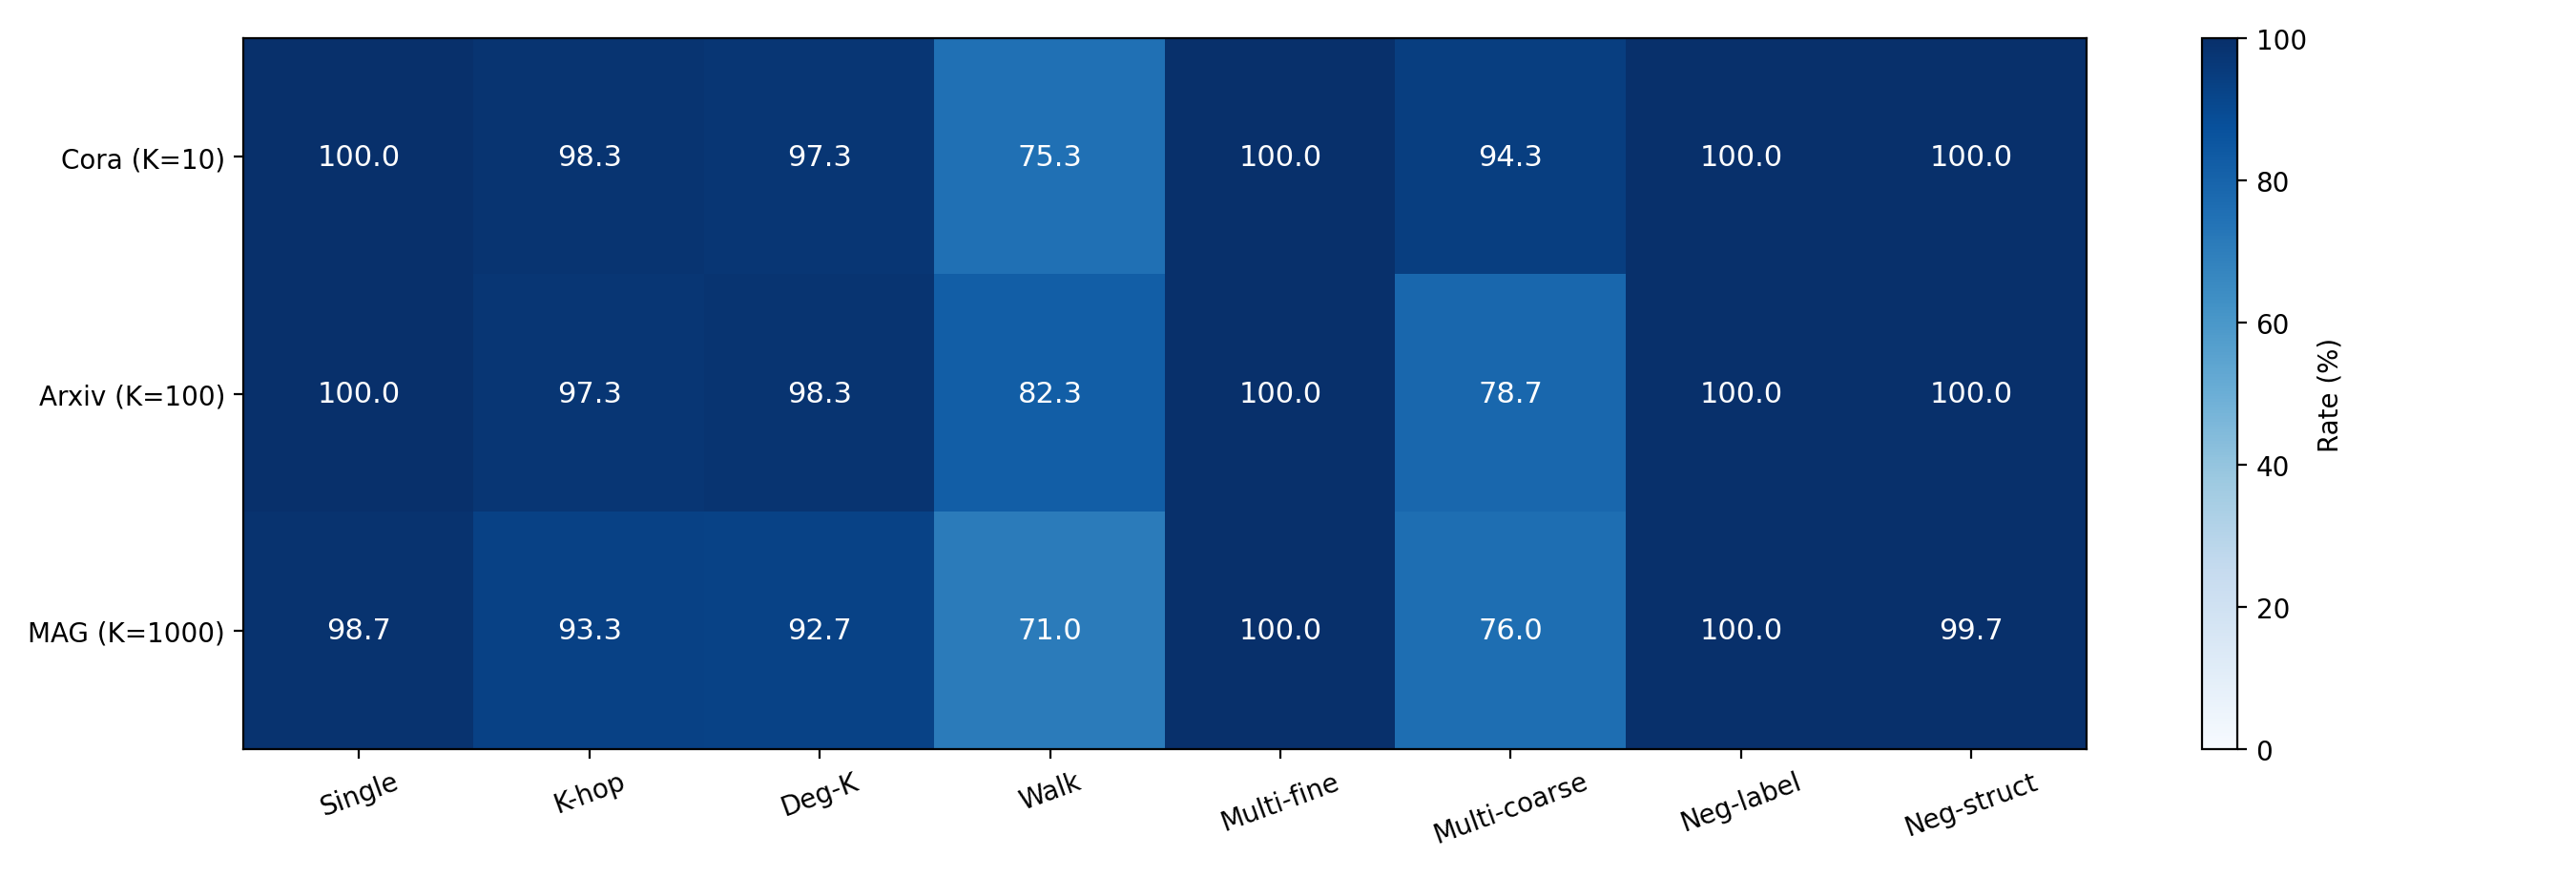
\includegraphics[width=\textwidth]{fig_jigsaw_query_family_heatmap.png}
\caption{\textbf{Jigsaw query-family outcomes.} Positive families report exact-solve rate; negative families report correct no-match rate. All rows are at the matched half-partition budget ($K{=}10/100/1000$). Random-walk and multi-coarse are the hard families across \emph{all three} datasets (Walk $75/82/71\%$, Multi-coarse $94/79/76\%$ on Cora/Arxiv/MAG); single and multi-fine saturate, local K-hop families remain high but not perfect on MAG, and negatives are rejected at ${\approx}100\%$.}
\label{fig:query_family_heatmap}
\end{figure}

\begin{figure}[H]
\centering
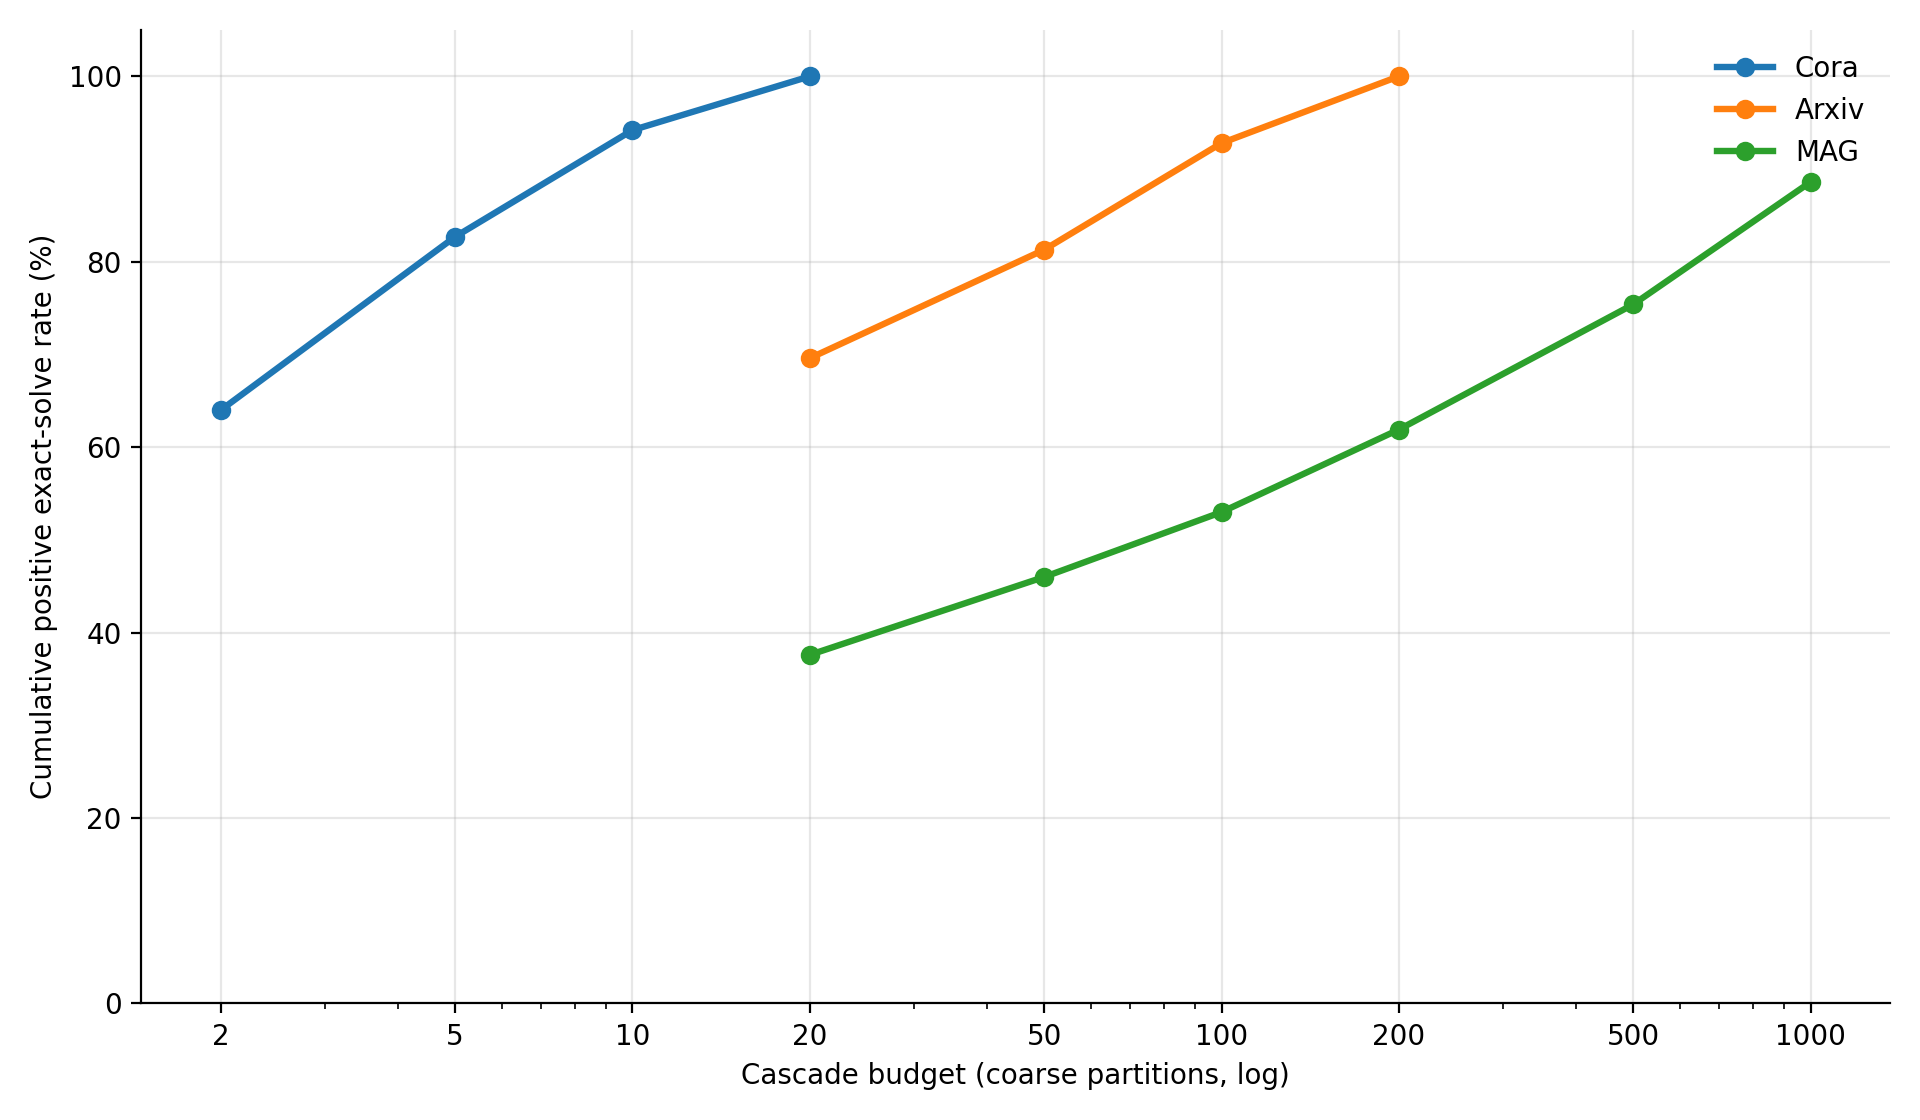
\includegraphics[width=0.80\textwidth]{fig_jigsaw_budget_curves.png}
\caption{\textbf{Solved-by-budget curves for Jigsaw.} Cora solves early because its candidate graphs are small and labels are strong. Arxiv benefits from budget expansion through 200. MAG continues improving through 1000, reflecting larger candidate regions and harder coverage.}
\label{fig:budget_curves}
\end{figure}

The budget curves sharpen the interpretation. On Cora the curve rises steeply ($64.0\%$ at budget 2 to $100\%$ by budget 20), so a handful of partitions decides most queries. Arxiv needs budget expansion to 200 before reaching its final positive solve rate, even though all policies eventually reach 100\%. MAG continues to improve through 500 and 1000, which means failures at small budgets are often not verifier unsoundness but insufficient candidate expansion. This supports the main design choice: a cascade should expose budget as a control knob rather than using one fixed candidate size for all queries.

\subsection{Label Selectivity: When Does Learned Retrieval Help?}
\label{sec:selectivity}

The production matrix uses vertex labels that are near-unique per node (md5 of the full feature vector). This flatters any \emph{exact-label} method: the classical label-coverage index (FeatureIndex) ranks a partition by how many of the query's labels it contains, which under near-unique labels is almost an oracle. It is therefore the strongest bounded retriever on this benchmark ($96.7\%$ solve; median worst-true-partition rank $104$ of $2{,}000$), ahead of the learned GNN ($88.6\%$; median rank ${\sim}900$). This is not a failure of the framework---it is a property of the benchmark's labels---and it motivates asking what happens when labels are \emph{not} near-unique.

We rerun the full MAG matrix with label granularity coarsened to the $39$ ground-truth classes (all families and sizes; $n{=}1800$ matched FeatureIndex queries). Two things change. First, the index's solve advantage \emph{disappears}: its median worst-true-partition rank degrades from $104$ to $1166$, and the complete coarse-label solve runs are statistically tied (FeatureIndex $63.4\%$; learned GNN variants $63$--$64\%$). Second, on retrieval the learned retriever has better worst-true-partition ranks in each family (Table~\ref{tab:selectivity}), because its embedding ranking is label-independent while the index's is not. The crossover is clean on ranking: \textbf{under near-unique labels the exact-label index dominates; under coarse, realistic labels the learned retriever is the better partition localizer, though not a solve-rate winner.} The planted-benchmark labels are the artifact, not the retriever. We are precise about the evidence: the retrieval crossover is \emph{model-independent}, since partition ranking uses the label-agnostic embedding and therefore holds for the deployed checkpoint; the end-to-end solve figures are corroborating only, because candidate size, timeouts, and false positives are genuinely label-dependent once pruning and the exact verifier consume labels.

\begin{table}[H]
\centering
\caption{\textbf{Label-selectivity crossover (MAG, coarse $39$-class labels, $n{=}1800$ matched).} Per-family retrieval quality: median worst-true-partition rank of $2{,}000$ (lower is better) and FullCov@$1000$. Under coarse labels the learned retriever has better per-family ranks than the classical index---the inverse of the near-unique-label regime---but complete solve rates are tied, and both are near-random on spatially-extended families (k-hop, degree-k-hop, random-walk).}
\label{tab:selectivity}
\small
\setlength{\tabcolsep}{6pt}
\begin{tabular}{lcccc}
\toprule
 & \multicolumn{2}{c}{\textbf{Learned (GNN)}} & \multicolumn{2}{c}{\textbf{FeatureIndex}} \\
\cmidrule(lr){2-3}\cmidrule(lr){4-5}
\textbf{Family} & \textbf{Med.\ rank} & \textbf{FullCov@1k} & \textbf{Med.\ rank} & \textbf{FullCov@1k} \\
\midrule
Single        & \textbf{7}    & 99\%  & 10   & 96\% \\
Multi-fine    & \textbf{3}    & 100\% & 6    & 99\% \\
Multi-coarse  & \textbf{747}  & 66\%  & 865  & 60\% \\
Degree-K-hop  & \textbf{1684} & 22\%  & 1800 & 10\% \\
K-hop         & \textbf{1697} & 16\%  & 1804 & 8\% \\
Random-walk   & \textbf{1783} & 11\%  & 1813 & 8\% \\
\bottomrule
\end{tabular}
\end{table}

\paragraph{The crossover generalizes, and it defines a portfolio.} The same inversion holds on Cora and OGBN-Arxiv (Table~\ref{tab:selectivity_xd}), and it tracks a single statistic computable \emph{offline}---the median number of partitions a label spans (Cora feature labels $1$, class labels $12$; Arxiv feature $1$, class $124.5$). Under near-unique feature labels the classical index is near-oracle: it \emph{ties} the learned retriever on contained families (single, multi-fine) and beats it on the harder families and overall (Cora overall median worst-true-partition rank $2$ vs.\ $5$; Arxiv $4$ vs.\ $44$). Under realistic class labels the index collapses toward random (Arxiv median $104$ of $200$), while the learned retriever degrades gracefully and has the better rank in \emph{every} family (Cora $5$ vs.\ $7$; Arxiv $44$ vs.\ $104$; per-query sign test $p<10^{-30}$ in both label regimes, $n{=}540$ each). Jigsaw therefore \emph{selects} its bounded retriever by label selectivity---high selectivity routes to FeatureIndex, low selectivity to the learned retriever---a deployable, non-oracle portfolio, since selectivity is a property of the graph and its labeling, not of the answer. On MAG the portfolio is corroborated end-to-end (FeatureIndex $96.7\%$ vs.\ learned $88.6\%$ solve at near-unique labels); on Cora and Arxiv it is a localization (retrieval-rank) result, as we did not run the exact solver there. The portfolio resolves the \emph{label-regime} axis only: spatially-extended queries stay hard for every retriever, as the next paragraph shows.

\begin{table}[H]
\centering
\caption{\textbf{Label-selectivity crossover across datasets.} Overall median worst-true-partition rank (lower is better; retrieval-only, identical queries, $n{=}540$ per dataset). Under near-unique \emph{feature} labels the classical index wins; under realistic \emph{class} labels the learned retriever wins. Median partitions/label quantifies selectivity. MAG ($2{,}000$ partitions) shows the same inversion at scale (Table~\ref{tab:selectivity}).}
\label{tab:selectivity_xd}
\small
\setlength{\tabcolsep}{6pt}
\begin{tabular}{lcccc}
\toprule
 & \multicolumn{2}{c}{\textbf{FeatureIndex}} & \textbf{Learned} & \textbf{Parts/label} \\
\cmidrule(lr){2-3}
\textbf{Dataset (parts)} & \textbf{feature} & \textbf{class} & \textbf{(any label)} & \textbf{feat / class} \\
\midrule
Cora ($20$)    & \textbf{2} & 7   & 5  & $1$ / $12$ \\
Arxiv ($200$)  & \textbf{4} & 104 & 44 & $1$ / $124.5$ \\
\bottomrule
\end{tabular}
\end{table}

The same experiment exposes the learned retriever's genuine limitation. It localizes \emph{contained} queries almost perfectly (single median rank $7$, multi-fine $3$) but is near-random on \emph{spatially-extended} queries (k-hop $1697$, degree-k-hop $1684$, random-walk $1783$ of $2{,}000$). The cause is structural: the current embedding geometry does not put every peripheral partition of a diffuse walk or large k-hop ball near the query, so FullCov---which requires \emph{every} one---fails. This is \emph{not} fixed by more training: the deployed walk-aware checkpoint has essentially identical per-family ranks (k-hop $1699$, random-walk $1751$), because retrieval ranking is label-independent and the walk-aware objective reshaped the training distribution, not the query representation. Nor is it fixed by any inference-time remedy we tested (Table~\ref{tab:probes}): subquery multi-vector MaxSim, finer partition parents, one- and two-hop fine-level overlap, dual-granularity late interaction, and coarse diffusion all leave FullCov@1000 within ${\approx}2$ points on the spatial families (best gain ${\approx}{+}2.3$), and a coarse neighbor-stitch expansion is actively harmful. The reason is structural: the MAG partition graph is high-degree even at fine granularity---a coarse partition borders a median $948$ of $2{,}000$ others and a fine partition a mean $568$ of $10{,}000$---so neighborhood-following broadens the candidate rather than tracing the query footprint. The high solve rates on these families in Table~\ref{tab:production_matrix} are thus carried by overlap stitching and exact-label pruning, not by retrieval. The open problem is representational: current embeddings do not discriminate spatially-extended regions at \emph{any} partition granularity, so the remaining plausible path is coverage/footprint-aware \emph{supervision} (a retrain), not an inference-time aggregation trick.

\begin{table}[H]
\centering
\caption{\textbf{Inference-time remedies do not recover coverage on spatially-extended MAG queries.} FullCov@$1000$ (\%) on the same $1{,}800$ held-out queries; a genuine fix needs ${\ge}{+}20$. Best gain is ${\approx}{+}2.3$ (coarse diffusion). A coarse neighbor-stitch expansion is omitted: it was actively harmful ($-8$ to $-13$).}
\label{tab:probes}
\small
\setlength{\tabcolsep}{5pt}
\begin{tabular}{lrrr}
\toprule
\textbf{Method} & \textbf{k-hop} & \textbf{degree-k-hop} & \textbf{random-walk} \\
\midrule
Single-vector (current)            & 14.7 & 17.3 & 9.0 \\
Subquery MaxSim (query-only)       & 14.3 & 17.7 & 8.0 \\
Finer partition parent             & 12.7 & 16.7 & 8.3 \\
Fine-level overlap (1-hop)         & 13.3 & 17.3 & 10.0 \\
Fine-level overlap (2-hop)         & 13.3 & 18.3 & 9.3 \\
Dual-granularity late interaction  & 12.7 & 16.0 & 8.7 \\
Coarse diffusion                   & 17.0 & 19.7 & 10.3 \\
\bottomrule
\end{tabular}
\end{table}

\subsection{Candidate-Shrinkage Cascade and Selective Overlap}
\label{sec:shrinkage}

A natural objection to retrieval-constrained verification is that if one-hop overlap is broad, the partition boundary may not be doing real work -- the system could be expanding to most of the graph and relying on pruning. We test this directly by measuring the per-query cascade
\[
\text{full graph} \to \text{overlap} \to \text{signature} \to \text{label-pruned} \to \text{solver components},
\]
on 14{,}400 MAG queries (10{,}800 positives) from the generic-mix-encoder run, at the budget each query is decided on (Figure~\ref{fig:shrinkage}). Three facts emerge.

\textbf{(1) Overlap is broad, but partition ranking still removes most of the graph.} The median union of selected-partition overlaps is 59\% of MAG for Jigsaw (vs.\ 73--83\% for mean-feature, random, and topology retrieval). After identical pruning, however, Jigsaw's candidate is a median 84.5K nodes versus 544K for FilterAll (medians; the production matrix reports means, 138.1K vs 443.8K), which performs no partition selection -- a $6.4\times$ reduction attributable to ranking alone. The boundary is blunt at the overlap stage but the ranking it feeds is not wasted.

\textbf{(2) All recall loss occurs at the overlap stage; pruning is coverage-lossless.} This is not merely empirical but a property of the pruning operator, which we state precisely.

\begin{proposition}[Lossless pruning]
\label{prop:lossless}
Let the pruning token $\sigma(\cdot)$ be a node attribute that the matching semantics preserve, i.e.\ any valid embedding $\phi$ of $Q$ into $G$ satisfies $\sigma(\phi(q))=\sigma(q)$ for every query node $q$ (vertex-labelled matching, with $\sigma$ derived from node type and feature labels). Prune the candidate $G_C$ to $G_C'=\{v\in G_C : \sigma(v)\in \sigma(V_Q)\}$. Then for any embedding $\phi$ with $\phi(V_Q)\subseteq G_C$, we have $\phi(V_Q)\subseteq G_C'$. Hence pruning preserves node coverage: $\mathrm{FullCov}$ is unchanged.
\end{proposition}
\emph{Proof.} For $q\in V_Q$, $\sigma(\phi(q))=\sigma(q)\in\sigma(V_Q)$, so $\phi(q)$ satisfies the keep condition and is retained. Thus every matched node survives. $\square$

The signatures used in the cascade (node type $\times$ feature-bit hashes) and the exact label filter are such attribute invariants, so Proposition~\ref{prop:lossless} applies; a \emph{degree}-based token would not be matching-invariant ($\deg(\phi(q))\ge\deg(q)$ only), which is why the pipeline prunes on attributes, not degree. Empirically this holds exactly: for every policy the planted-match survival rate after overlap equals that after pruning (Jigsaw $87\%$ both before and after in this generic-encoder diagnostic, whose end-to-end solve is $86.0\%$), so the solve ceiling is set entirely by whether the retrieved-plus-overlapped region \emph{contains} the match. All retrieval-recall loss is localized to the overlap stage, never the pruning stage.

\textbf{(3) Latency is dominated by candidate construction, not solving.} Mean per-query candidate-build time is 3.4\,s for Jigsaw and 5.5\,s for FilterAll, against 0.25\,s of exact solving. (These means come from the generic-encoder shrinkage diagnostic; the production-matrix totals also include retrieval and use the walk-aware encoder, so they are not directly additive.) The exact verifier is cheap; assembling and pruning the broad overlap union is the cost. This is why Jigsaw's total latency does not yet beat FilterAll despite a $3.2\times$ smaller mean candidate.

\begin{figure}[H]
\centering
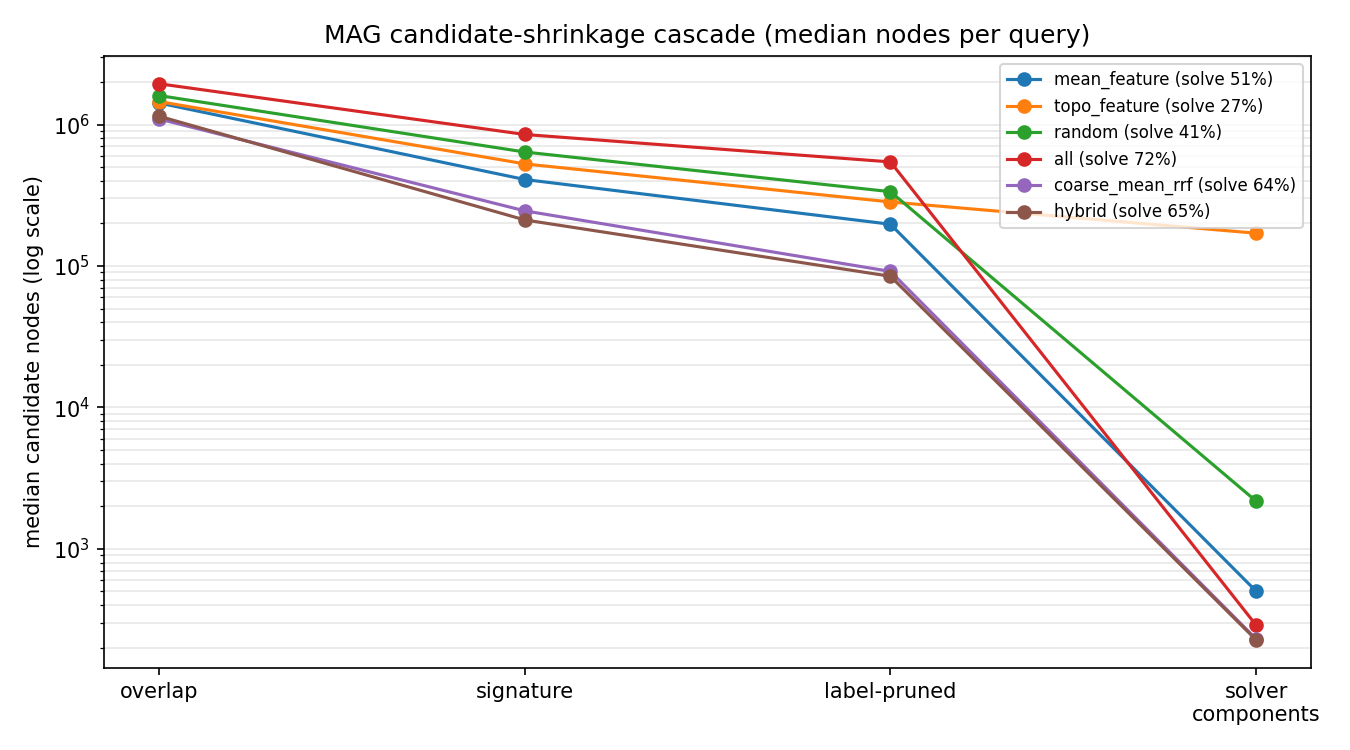
\includegraphics[width=0.86\textwidth]{fig_candidate_shrinkage_mag.png}
\caption{\textbf{MAG candidate-shrinkage cascade (median nodes per query, log scale).} Each policy's candidate is tracked through overlap, signature, label pruning, and component decomposition. Learned retrieval (Jigsaw) and Mean-RRF reach much smaller solver inputs than uninformed policies, and far smaller than FilterAll, even though all share the same lossless pruning.}
\label{fig:shrinkage}
\end{figure}

\paragraph{Why broad overlap is mostly wasted, and the selective-overlap fix.}
The breadth of one-hop overlap is not buying recall. A controlled probe over the cached MAG index shows that when retrieval misses a true partition, one-hop overlap recovers it for 94\% of K-hop queries but only 62\% of random-walk queries: overlap reaches only the \emph{boundary} nodes of retrieved partitions, never the interior of a fully unselected partition. The same mechanism explains the random-walk weakness in Section~\ref{sec:family} (a diffuse walk's missed mid-path partitions are not boundary-adjacent to retrieved ones). Broad overlap therefore inflates candidate size in the common case where retrieval already succeeded, without repairing the misses. This motivates \emph{selective overlap}: instead of admitting every bordering partition's boundary nodes, expand each selected partition only to its highest-support neighbors (ranked by bridge boundary count) and/or to label-compatible nodes. Because selective overlap trims only overlap nodes and never partition interiors, it preserves the recall that partition selection provides while shrinking the dominant candidate-build cost. In the cached-index probe (pooled over the four query families), capping each partition to its eight strongest neighbors cuts the overlap union by ${\approx}3.1\times$, label-compatible expansion by ${\approx}5.0\times$, and the two combined by over $6\times$, at no cost in candidate \emph{size} (the probe validates the volume reduction; a recall-preserving claim requires the aligned-hierarchy re-run we leave to future work). We provide selective overlap as configurable operators (\texttt{--overlap-max-parts}, \texttt{--overlap-min-support}, \texttt{--overlap-label-compatible}) and identify it as the principal systems lever for closing the FilterAll gap at lower latency. Crucially, reducing node volume is the \emph{only} lever available: candidate construction is volume-bound, not algorithm-bound -- replacing the set-union with a vectorized tensor union gives no speedup (it is verified identical but $0.5$--$0.9\times$ as fast), so the dominant build cost falls only when the number of admitted nodes falls.

\subsection{What the Ablations Establish}

The Arxiv retrieval ablation establishes the learning contribution: optimizing FullCov directly improves coverage at every fixed budget in Table~\ref{tab:loss_ablation}. The production design ablations in Table~\ref{tab:design_ablation} and Figure~\ref{fig:design_ablation} establish the systems contribution. These rows are diagnostic slices rather than a replacement for the full production matrix: some ablations were run only on positives or only on negatives because they test a specific mechanism.

\begin{table}[H]
\centering
\caption{\textbf{Operator-necessity ablation (shared 48-query set per dataset).} Each row disables one cascade operator; rows measure \emph{relative} necessity on one shared query set, so absolute rates are diagnostic, not the production matrix. The two datasets stress \emph{different} operators. On MAG, removing \textbf{overlap} halves the positive solve rate (boundary-crossing matches cannot complete without the one-hop halo). On Arxiv -- small enough that every variant still solves $100\%$ -- the story is candidate size: removing \textbf{signatures} explodes the candidate domain ${\sim}75\times$ ($94{\to}7{,}081$ nodes), showing why exact verification needs typed pruning at scale. Overlap is a no-op on Arxiv and signatures are inert on MAG: each operator earns its keep where the graph stresses it.}
\label{tab:design_ablation}
\scriptsize
\setlength{\tabcolsep}{5pt}
\resizebox{\textwidth}{!}{%
\begin{tabular}{lrrrr}
\toprule
 & \multicolumn{2}{c}{\textbf{OGBN-MAG}} & \multicolumn{2}{c}{\textbf{OGBN-Arxiv}} \\
\cmidrule(lr){2-3}\cmidrule(lr){4-5}
\textbf{Variant} & \textbf{Solve \%} & \textbf{Cand.} & \textbf{Solve \%} & \textbf{Cand.} \\
\midrule
Full Jigsaw    & 88.9          & 64.0K & 100.0 & 94 \\
No overlap     & \textbf{44.4} & 49.9K & 100.0 & 97 \\
No signature   & 88.9          & 64.0K & 100.0 & \textbf{7{,}081} \\
No components  & 63.9          & 65.2K & 100.0 & 94 \\
No exact-label & 52.8          & 100.7K  & 100.0 & 223 \\
\bottomrule
\end{tabular}}
\end{table}

\begin{figure}[H]
\centering
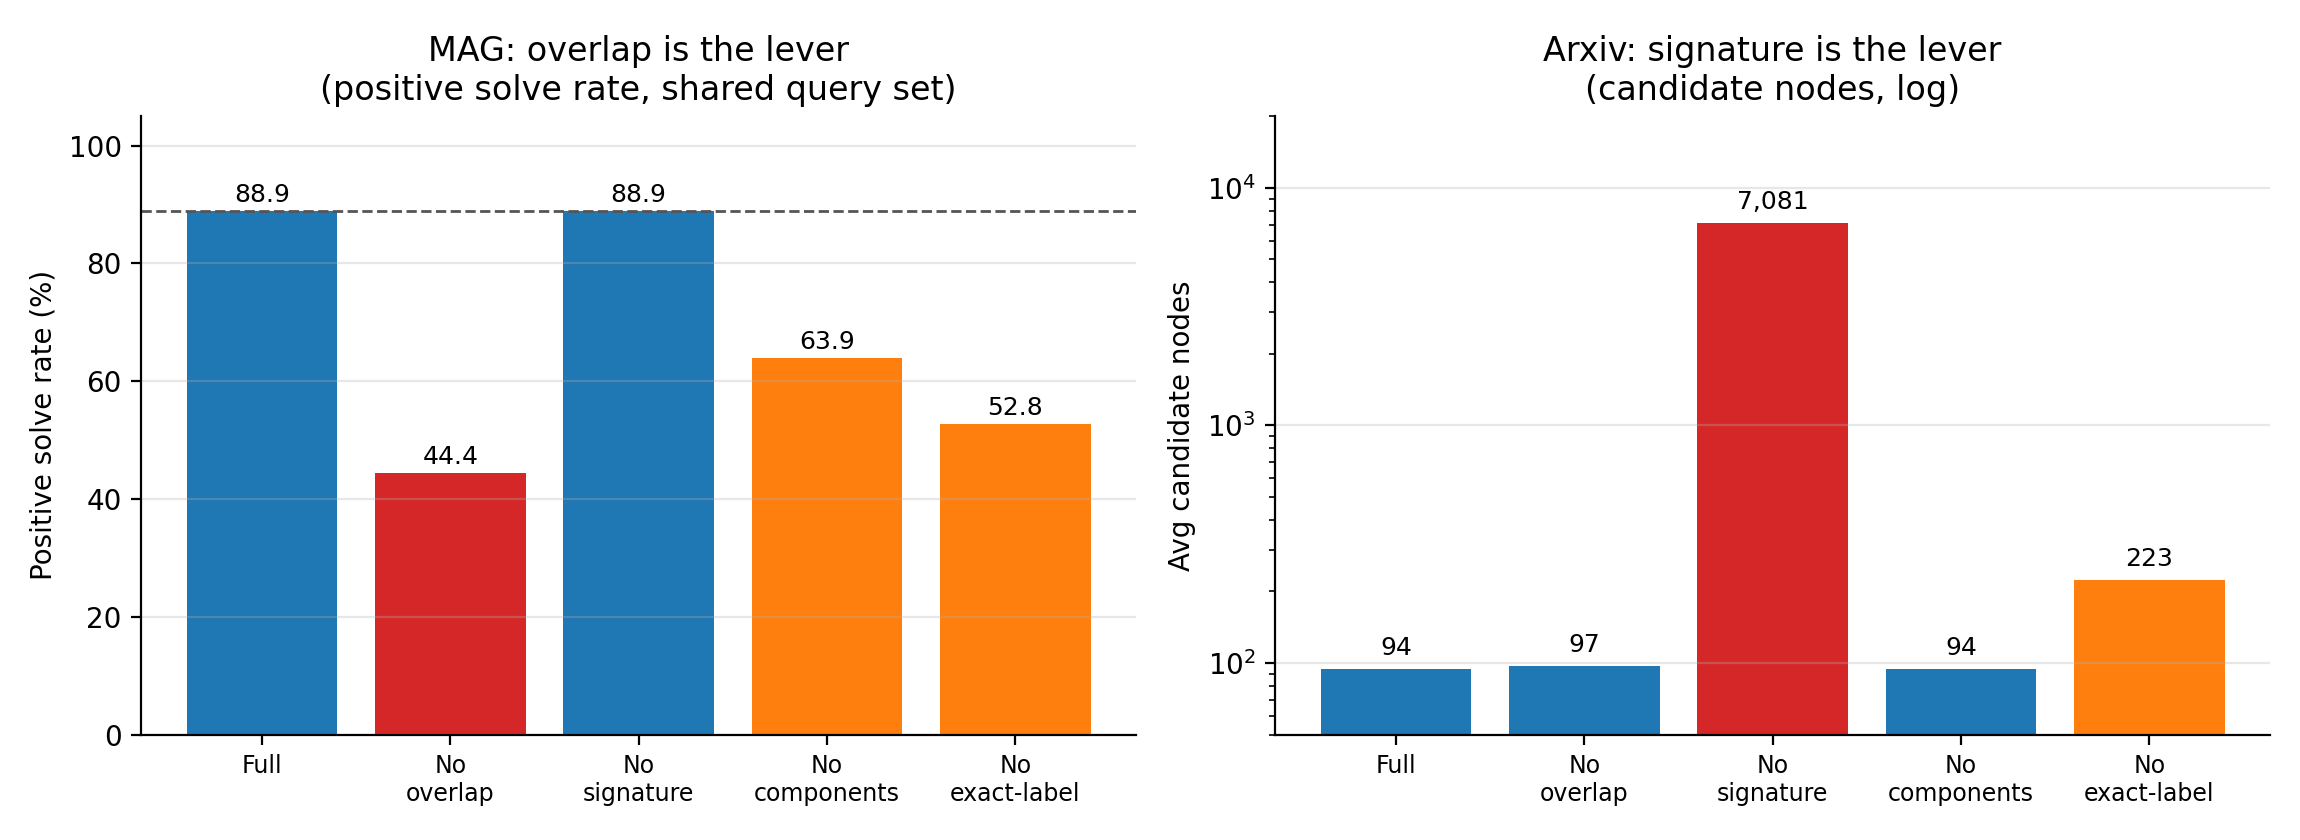
\includegraphics[width=0.78\textwidth]{fig_design_ablation.png}
\caption{\textbf{Operator necessity is dataset-dependent.} \emph{Left:} on MAG, disabling overlap halves the positive solve rate ($88.9{\to}44.4\%$) -- overlap recovers boundary-crossing matches at scale; signatures are inert. \emph{Right:} on Arxiv, disabling signatures explodes the candidate domain ${\sim}75\times$ ($94{\to}7{,}081$ nodes, log axis) while overlap is a no-op. Each operator is a pillar on the graph that stresses it.}
\label{fig:design_ablation}
\end{figure}

The two ablations tell one story: \emph{the cascade's operators are dataset-dependent, and both are necessary because different graphs stress different ones}. On MAG (2{,}000 partitions, boundary-crossing queries) \textbf{overlap} is the pillar -- removing the one-hop halo halves the solve rate ($88.9{\to}44.4\%$), because matches that straddle a partition cut cannot complete without it; signatures, by contrast, are \emph{inert} on MAG (identical solve and candidate size with and without, $88.9\%$ / $64.0$K), since the flattened heterogeneous graph gives the typed fingerprint little to discriminate. On Arxiv the roles invert: overlap is a no-op ($94{\to}97$ candidate nodes -- retrieval already covers the small, dense match), while \textbf{signatures} are the pillar -- removing them inflates the candidate domain ${\sim}75\times$ ($94{\to}7{,}081$ nodes), which is exactly the candidate explosion an exact verifier cannot afford at scale even when (as here) the small graph still solves. Across both, exact-label pruning matters for candidate size and negative rejection (Arxiv $94{\to}223$; MAG solve $88.9{\to}52.8\%$ as un-pruned candidates time out), and component decomposition helps the MAG solve rate ($88.9{\to}63.9\%$ without it) by keeping solver inputs small. The lesson for the production setting is that no single operator can be dropped: the overlap-cascade must carry all of them because the operator that is idle on one dataset is decisive on another.

\subsection{Model-Variant Diagnostics}

The final benchmark bundle also preserves diagnostic rows that are not counted in the canonical production matrix. For Arxiv, continuation/v7 rows show that extending training can change retrieval behavior, but the selected production claim uses the base \texttt{arxiv} model for a balanced two-seed matrix. For MAG, both \texttt{mag\_rgcn\_best} and \texttt{mag\_rgcn\_final} were benchmarked for neural and Mean-RRF rows; the production matrix uses \texttt{mag\_rgcn\_best} because validation selected it by FullCov. The \texttt{mag\_rgcn\_final} rows are retained as diagnostic model ablations rather than silently averaged into production.

\subsection{Negative Queries and Soundness}

Jigsaw never accepts a match from the neural model alone. The only accepting step is Glasgow verification. Negative-label and negative-structure queries therefore test the practical no-match behavior of the candidate construction and exact verifier. Across the final paper bundle, audited no-match accuracy is 100.0\% for Cora and Arxiv summaries and 99.7--99.8\% for selected MAG rows, with at most one false positive per method in the selected MAG summaries. These false positives are not verifier hallucinations; they indicate that the synthetic negative construction can still produce a valid exact match in the data graph, a known risk when generating negatives by local perturbation rather than by a global non-isomorphism certificate.

This distinction matters for reviewer interpretation. A returned Glasgow mapping is a real isomorphism inside the candidate graph. If the negative generator perturbs a query but the large data graph happens to contain another matching structure, the solver is behaving correctly even though the benchmark label expected no match. Therefore we report false positives as benchmark-level failures, not as neural hallucinations. A stronger future negative benchmark would certify non-existence globally, but that is precisely the expensive exact problem that motivates retrieval-constrained verification.

\section{Discussion and Limitations}
\label{sec:limits}

Jigsaw should be read as an exact-verification system with a learned boundary, not as a proof of global completeness. If retrieval misses a necessary region, the solver cannot recover the planted match. FullCov makes that failure mode measurable. The current system is strongest for static attributed graphs and repeated query workloads, where partitioning, embedding, and FAISS indexing can be amortized. Cora and Arxiv do not demonstrate a large end-to-end neural advantage because exact labels and pruning already dominate once coverage is sufficient. MAG is the main production dataset where retrieval policies separate: FeatureIndex is strongest under near-unique labels, while learned retrieval becomes the better localizer as labels coarsen. The corrected connected-query reruns also clarify an earlier benchmark artifact: disconnected multi-region rows should not be used to claim that realistic cross-boundary queries fail. FilterAll is still valuable as an upper bound, but it is not a scalable replacement for retrieval.

The main empirical limitation is comparison scope. We compare against classical feature- and structure-index rankers (the MeanFeat and TopoFeat policies, GraphGrep/gIndex-style filters), a no-retrieval exact control (full-graph Glasgow, which solves $0/15$ MAG queries and establishes that retrieval is a prerequisite at scale), an exhaustive FilterAll upper bound, and uninformed feature/random/topology retrievers. Learned node-alignment matchers such as NeuroMatch and GLSearch are not applicable baselines at this scale and setting: they are trained and evaluated on small graphs (hundreds of nodes) with the query \emph{contained} in a single target, and emit node/pair scores with no scalable route to million-node targets or to queries that span many partitions -- a different problem class, not merely an unimplemented comparison. We do benchmark scalable filter-and-verify matchers (CFL-Match, DP-iso, GQL) directly (Table~\ref{tab:external}): they confirm exact matching is feasible on Cora/Arxiv and on MAG once the whole graph is loaded, so our infeasibility claim is scoped to the CP-based Glasgow solver Jigsaw uses (0/15 on full MAG) and to the memory and low-selectivity regimes where these matchers degrade (12/27 at coarse labels), not a blanket impossibility of exact matching. The residence axis itself has out-of-core and distributed precedents (DUALSIM~\cite{ref_dualsim}, STwig/Trinity~\cite{ref_trinity}, G-thinker~\cite{ref_gthinker}); Jigsaw differs in bounding residence by \emph{learned region relevance} on a single machine rather than by streaming or sharding the whole graph, and we make no claim of outperforming those systems---only of exposing a tunable memory budget a CP verifier alone cannot. This benefit must also be weighed against offline cost (METIS partitioning, encoder training, and embedding the partition bank are one-time but nontrivial), so the memory argument is strongest for graphs that cannot be held resident, or for multi-tenant and cold-start serving, rather than for a single amortizable load over a static graph. A scoped GNN-PE public-release diagnostic is reported below. A second limitation is negative-query certification: the released negative families are audited synthetic no-match tests, not a global proof that no embedding exists anywhere in the full graph. This is why the paper reports false positives and no-match accuracy instead of claiming theorem-level global negative completeness. A third is workload: queries are planted connected subgraphs rather than an external pattern workload, and evaluation is on static single graphs where the index amortizes. On these label-rich planted benchmarks several policies localize the candidate well once coverage is met, so we do not claim the learned retriever dominates cheaper ones on \emph{recall}; its role is to make the candidate small and memory-bounded, and FullCov is what secures coverage on the hard families where cheaper policies fail (Section~\ref{sec:family}). Establishing a regime where a learned retriever is also decisive on recall would need harder, weakly-labeled or non-planted query workloads, which we leave to future work.

\paragraph{GNN-PE public-release diagnostic.}
We also ran the released GNN-PE pipeline on Cora: its bundled self-test passes, but after class-label export, build/serialization repairs, and an $e=128$ stress test it recovered only $7/24$ planted positives at $e=4$ and $5/24$ at $e=128$ ($0/6$ at size 100) -- a higher embedding dimension did not help. The released executable builds path/label embeddings and indexes directly and exposes no separate supervised training step for these runs, so this is a public-release feasibility result, not a full-recipe reproduction; the pipeline remains unusable for our planted-query protocol without deeper upstream changes.

\begin{table}[H]
\centering
\caption{\textbf{External baselines on planted queries}, complementing the internal retrieval-policy comparison of Table~\ref{tab:production_matrix}. \emph{Direct} is the CP-based Glasgow solver with no retrieval; \emph{GNN-PE} is the released public implementation on Cora (Section~\ref{sec:limits}). Classical filter-and-verify matchers (CFL-Match, DP-iso, GQL) solve Cora/Arxiv and solve MAG \emph{once the whole graph is loaded} at high label selectivity, but require the full graph resident and collapse at coarse labels.}
\label{tab:external}
\small
\resizebox{\textwidth}{!}{%
\begin{tabular}{lll}
\toprule
\textbf{Method} & \textbf{Setting} & \textbf{Planted-query result} \\
\midrule
Direct Glasgow (no retrieval) & Cora / Arxiv / MAG & 15/15 \; / \; 0/15 \; / \; 0/15 \\
GNN-PE (public release) & Cora, $e{=}4$ / $e{=}128$ & 7/24 \; / \; 5/24 \ \ ($0/6$ at $n{=}100$) \\
CFL-Match / DP-iso / GQL & Cora / Arxiv & 100\% \, / \, 100\% \ ($2.35\times$ slower than Jigsaw, Cora) \\
CFL-Match / DP-iso / GQL & MAG, whole graph resident & 27/27 high-selectivity; \textbf{12/27} at coarse labels \\
\midrule
\textbf{Jigsaw} & MAG (fair budget $K{=}1000$) & \textbf{88.6\%}, bounded memory \\
\bottomrule
\end{tabular}}
\end{table}

\section{Conclusion}

Jigsaw connects learned graph retrieval and exact subgraph verification through a measurable coverage condition. The FullCov objective improves the probability that all required regions are retrieved; overlap and pruning make exact verification tractable; and the completed Cora, Arxiv, and MAG matrix clarifies both the promise and the boundary of the approach. The strongest conclusion is not that a neural retriever wins: Jigsaw is \emph{retriever-agnostic}, and which retriever is best depends on label selectivity---a classical label index is strongest under the near-unique labels of planted benchmarks, while learned retrieval becomes the better localizer as labels coarsen. The contribution is the system: exact subgraph verification made usable on large static graphs under a bounded memory footprint, retrieving and pruning candidate partitions rather than ever materializing the whole graph. Two axes remain. The \emph{label-regime} axis is already handled: Jigsaw selects its bounded retriever by offline label selectivity---a classical index under near-unique labels, the learned retriever under realistic ones (confirmed on Cora, Arxiv, and MAG). Making retrieval decisive on \emph{spatially-extended} queries stays open: inference-time remedies at both partition granularities did not recover coverage, pointing to coverage/footprint-aware representation learning rather than inference-time aggregation.

\begin{thebibliography}{25}

\bibitem{ref_glasgow}
McCreesh, C., Prosser, P., Trimble, J.: The Glasgow Subgraph Solver: Using Constraint Programming to Tackle Hard Subgraph Isomorphism Problem Variants. In: CP 2020, LNCS, vol. 12333, pp. 316--333. Springer (2020)

\bibitem{ref_gin}
Xu, K., Hu, W., Leskovec, J., Jegelka, S.: How Powerful are Graph Neural Networks? In: ICLR (2019)

\bibitem{ref_vf2}
Cordella, L.P., Foggia, P., Sansone, C., Vento, M.: A (Sub)Graph Isomorphism Algorithm for Matching Large Graphs. IEEE TPAMI \textbf{26}(10), 1367--1372 (2004)

\bibitem{ref_faiss}
Johnson, J., Douze, M., J\'egou, H.: Billion-Scale Similarity Search with GPUs. IEEE Trans. Big Data \textbf{7}(2), 535--547 (2021)

\bibitem{ref_metis}
Karypis, G., Kumar, V.: A Fast and High Quality Multilevel Scheme for Partitioning Irregular Graphs. SIAM J. Sci. Comput. \textbf{20}(1), 359--392 (1998)

\bibitem{ref_ogb}
Hu, W., et al.: Open Graph Benchmark: Datasets for Machine Learning on Graphs. In: NeurIPS (2020)

\bibitem{ref_garey}
Garey, M.R., Johnson, D.S.: Computers and Intractability: A Guide to the Theory of NP-Completeness. W.H. Freeman (1979)

\bibitem{ref_ri}
Bonnici, V., Giugno, R., Pulvirenti, A., Shasha, D., Ferro, A.: A Subgraph Isomorphism Algorithm and Its Application to Biochemical Data. BMC Bioinformatics \textbf{14}(Suppl 7), S13 (2013)

\bibitem{ref_lad}
Solnon, C.: AllDifferent-Based Filtering for Subgraph Isomorphism. Artificial Intelligence \textbf{174}(12--13), 850--864 (2010)

\bibitem{ref_cora}
Sen, P., Namata, G., Bilgic, M., Getoor, L., Galligher, B., Eliassi-Rad, T.: Collective Classification in Network Data. AI Magazine \textbf{29}(3), 93--106 (2008)

\bibitem{ref_neuromatch}
Ying, R., et al.: Neural Subgraph Matching. arXiv:2007.03092 (2020)

\bibitem{ref_gnnpe}
Ye, Y., Lian, X., Chen, M.: Efficient Exact Subgraph Matching via GNN-based Path Dominance Embedding. Proc. VLDB Endow. \textbf{17}(7), 1628--1641 (2024)

\bibitem{ref_glsearch}
Liu, Y., et al.: GLSearch: Maximum Common Subgraph Detection via Learning to Search. In: ICML (2021)

\bibitem{ref_nsic}
Liu, X., Pan, H., He, M., Song, Y., Jiang, X., Shang, L.: Neural Subgraph Isomorphism Counting. In: KDD (2020)

\bibitem{ref_turboiso}
Han, W.S., Lee, J., Lee, J.H.: TurboISO: Towards Ultrafast and Robust Subgraph Isomorphism Search in Large Graph Databases. In: SIGMOD, pp. 337--348 (2013)

\bibitem{ref_cflmatch}
Bi, F., Chang, L., Lin, X., Qin, L., Zhang, W.: Efficient Subgraph Matching by Postponing Cartesian Products. In: SIGMOD, pp. 1199--1214 (2016)

\bibitem{ref_daf}
Han, M., Kim, H., Gu, G., Park, K., Han, W.S.: Efficient Subgraph Matching: Harmonizing Dynamic Programming, Adaptive Matching Order, and Failing Set Together. In: SIGMOD, pp. 1429--1446 (2019)

\bibitem{ref_vf3}
Carletti, V., Foggia, P., Saggese, A., Vento, M.: Challenging the Time Complexity of Exact Subgraph Isomorphism for Huge and Dense Graphs with VF3. IEEE Trans. Pattern Anal. Mach. Intell. \textbf{40}(4), 804--818 (2018)

\bibitem{ref_gsi}
Zeng, L., Zou, L., \"Ozsu, M.T., Hu, L., Zhang, F.: GSI: GPU-friendly Subgraph Isomorphism. In: ICDE, pp. 1249--1260 (2020)

\bibitem{ref_survey}
Sun, S., Luo, Q.: In-Memory Subgraph Matching: An In-depth Study. In: SIGMOD, pp. 1083--1098 (2020)

\bibitem{ref_dualsim}
Kim, H., Lee, J., Bhowmick, S.S., Han, W.-S., Lee, J., Ko, S., Jarrah, M.H.A.: DUALSIM: Parallel Subgraph Enumeration in a Massive Graph on a Single Machine. In: SIGMOD, pp. 1231--1245 (2016)

\bibitem{ref_trinity}
Sun, Z., Wang, H., Wang, H., Shao, B., Li, J.: Efficient Subgraph Matching on Billion Node Graphs. Proc. VLDB Endow. \textbf{5}(9), 788--799 (2012)

\bibitem{ref_gthinker}
Yan, D., Guo, G., Chowdhury, M.M.R., \"Ozsu, M.T., Ku, W.-S., Lui, J.C.S.: G-thinker: A Distributed Framework for Finding Qualified Subgraphs in a Big Graph with Load Balancing. In: ICDE (2020)

\end{thebibliography}
\end{document}
